\section*{Guide to the supplementary evidence}
The native-key protocols, alternative aggregation rules and information controls support the main claims. Secondary selector studies and scoring limitations are distinguished from independent confirmation.

\begin{center}\small
\begin{tabular}{>{\raggedright\arraybackslash}p{.55\linewidth}>{\raggedright\arraybackslash}p{.37\linewidth}}
\toprule
Question or evidence & Where to look\\
\midrule
Rule contrast, tie explanation, 288 native questions & Section~\ref{app:representation}\\
Selected-policy loss, 720 native questions & Section~\ref{app:native720}\\
Health gain versus stronger policy & Section~\ref{app:health}\\
One-answer versus five-answer generation & Section~\ref{app:contract}\\
Policy, budget and partner sensitivities & Sections~\ref{app:joint_policy}, \ref{app:allocation_budget}, \ref{app:partner_composition}\\
IRV, rank transfer and conditional diagnostics & Sections~\ref{app:irv}--\ref{app:conditional}\\
Membership ceilings, wrong-option controls and equal-budget screening & Section~\ref{app:review_followthrough}\\
Notation and replay instructions & Section~\ref{app:reader_card}\\
Clinical mapping and worst-case uncertainty & Sections~\ref{app:mapping}, \ref{app:representation}\\
Held-out predictor specification & Section~\ref{app:readability_detail}\\
Secondary selector interventions & Section~\ref{app:selector_detail}\\
Reproduction resources and serving limits & Section~\ref{app:repro}\\
\bottomrule
\end{tabular}
\end{center}


\section{Representation and native-answer confirmation protocols}\label{app:representation}
\subsection{Original 288-question representation study}
The representation question was selected after inspecting the earlier banks. Its separate protocol was frozen on 9 September 2026 before any new generation. Let $A_r=F_{M,r}-F_{H,r}$ for TRUE support and define the sole primary $C=A_{\mathrm{inclusion},5}-A_{\mathrm{first}}$. Native-key MedXpertQA is primary; MedEinst is a separate prespecified transport. The study does not generate new LLM-selector decisions. It tests transformations of saved five-answer lists, not prompting for one versus five answers.

\paragraph{Case selection.}
We exclude 3,902 previously used MedEinst IDs and 128 native IDs, normalized input matches and duplicate eligible inputs. Native sampling takes 96 hash-ranked questions in each of Diagnosis, Treatment and Basic Science. From 1,481 eligible MedEinst pairs, we select 32 short, 32 medium and 32 long pairs by hash rank, requiring each pair to differ by one line. This replaces the initially planned two-block frequency/length-balanced sample, whose second block was infeasible; the change preceded all model calls. The final sample is length-balanced but not transition-frequency-balanced: it contains 90 high-, five medium- and one low-frequency pairs. Neither historical IDs nor normalized inputs overlap with the analyzed sample.

\paragraph{Sampling and failures.}
Each case has two new banks, with independent request identities/seeds; provider determinism and independent internal randomness are not guaranteed. Per branch/bank, H takes eight Gemma calls and M shares its first two plus two calls to each other generator, giving 14 unique calls. There are $14\times2\times(288+2\times96)=13,440$ scheduled identities. Generators use the same five-answer contract, temperature 1, top-$p=.9$ and 384-token cap. Gemma, Llama and Ministral use OpenRouter; Qwen uses the official Qwen2.5-14B-Instruct checkpoint in BF16 through vLLM 0.10.2/transformers 4.55.2. An exact weight-revision hash was not returned. Every invalid slot receives at most one identical-payload retry; first valid output is retained and terminal failures remain empty. The protocol requires terminal failures to remain at or below 5\% in each source/model cell. All eight cells satisfy this threshold; the highest rate is 3.73\% (native Llama), with denominators in Table~\ref{tab:failure_cells}. Independent banks are averaged within case, and MedEinst branches within pair, before inference.

\paragraph{Rules and statistics.}
First-choice, inclusion, reciprocal rank, RR restricted to inclusion ties and truncated Borda are specified in the main text. Each call contributes once per normalized candidate at its best rank. Borda weights are $5,4,3,2,1$, with zero for absent candidates. Unresolved ties use expected uniform correctness. Transition accounting couples ties through a common uniform random candidate priority; unchanged winner sets cannot manufacture disagreements. The tie component is the H-minus-M accuracy gain from replacing inclusion by tie-aware frequency; subtracting it from $C$ leaves the tie-aware-versus-first allocation contrast. This is an accounting identity, not a mediation estimate.

The desired 95\% interval half-width was five percentage points. Old case-level standard deviations .41535 native and .24058 MedEinst imply approximate requirements of 266 and 89 cases under $n=(1.96s/.05)^2$; fixed 288/96 preserve task/length balance. No reduction was assumed from averaging banks. The primary uses 50,000 task-stratified native case bootstraps, seed 202609091733; MedEinst resamples whole pairs. Depths 2--4, other rules, bank differences, flips and decomposition are secondary pointwise summaries. Uncertainty conditions on benchmark keys or the frozen deterministic refinement/strict/exact-reference mapping algorithm, not clinical adjudication.

\paragraph{One held-out prediction check.}
A ridge predictor of case-level $C$ is fit only on the earlier native128. Its fixed rival inputs are M-minus-H candidate count divided by ten and rank-one vote concentration; an enriched model adds the H-minus-M inclusion-tie indicator. Inputs are standardized on training cases, ridge coefficient is one and the intercept is the training mean. This specification was frozen after new generation began but before fresh correctness was analyzed. It is a secondary held-out check, not pregeneration registration. The single comparison is paired fresh-native MSE reduction from adding the tie gap, with 50,000 task-stratified bootstrap resamples. A constant old-training-mean predictor is also retained. Prediction does not establish causal competence adjustment or an improved allocation policy.

\paragraph{Local reproduction.}
The exact protocol is \path{Protocols/REPRESENTATION_CONFIRMATION_2026_09_09.md}; schedules, raw attempts, source hashes, frozen dependencies and operational manifests are under \path{runs/representation_confirmation_2026_09_09/}. From the complete local project, run \path{code/representation_confirmation_20260909.py} with argument \texttt{analyze}, then \path{code/verify_representation_confirmation_20260909.py}; these consume stored outputs. The independent verifier reconstructs native options, rational-valued votes, all ten absolute rule/allocation cells, case/bank contrasts and the primary interval from raw output text. It does not adjudicate MedEinst labels. The saved-model prediction is evaluated with \path{code/predict_representation_boundary_20260909.py evaluate}. Do not run \texttt{setup}, \texttt{execute} or \texttt{freeze} to reproduce the saved analysis. The earlier rule integration and current figures are under \path{runs/maintrack_strengthening_2026_09_09/}. Dataset question text and credentials are not part of the manuscript-source archive.

\paragraph{Operational sensitivity.}
The saved-attempt audit verifies all 13,440 scheduled identities, at most two attempts per identity, identical retry payloads, and retention of the first valid output. A post-outcome complete-case sensitivity excludes any case with a failed generation: native $n=193$ gives $C=8.86$ points (95\% CI $[3.32,14.49]$); MedEinst $n=88$ gives $4.62$ $[.28,9.15]$. These exclude 95 native cases and eight pairs, change the sampled population and native task mixture, and do not replace the primary with empty failures retained. Retained native counts are 66 Diagnosis, 62 Treatment and 65 Basic Science. These sensitivity intervals use 50,000 unstratified whole-case resamples with seed 202609091733; the primary remains task-stratified. No additional calls were collected.

\paragraph{Mapping implementation and protocol discrepancy.}
The fresh transport map contains 3,607 candidate--reference relation types: 2,401 new and 1,206 reused. Of 2,846 strict-unresolved types, 2,388 are new. The frozen code also applies a separate refinement whitelist, crediting 24 strict-unresolved types (ten new, 14 reused). This conflicts with the protocol prose that newly unresolved relations remain uncredited. We preserve the original protocol, code and results and report the discrepancy: setting all new unresolved relations to zero gives $C=4.93$ points (95\% CI $[.87,9.17]$), compared with the implemented $4.85$ $[.77,9.08]$. Setting all strict-unresolved relations to zero gives $6.10$ $[2.01,10.38]$, identical here to strict/literal scoring. These fixed-rule checks leave the direction intact; they do not resolve arbitrary clinical relabeling.

The 3,607 types occur in 12,487 candidate--pool incidences; 6,760 incidences are unresolved. All 96 pairs contain unresolved candidates. The 24 refinement credits affect the case-level contrast in 19 pairs, and 171 unresolved types have nonzero overall contrast coefficients. A shared-relation binary stress bound is $[-26.34,29.85]$ points; this is a deterministic worst-case envelope, not a confidence interval or medically plausible adjudication. The native primary uses official option keys and is unaffected. The incidence and sensitivity audit is reproduced by \path{code/audit_latest_review_mapping_20260910.py} on the saved map and pools.

\paragraph{Resource closure.}
The fresh representation program attempted 13,440 scheduled identities with 13,845 raw attempts, including allowed retries. There are 13,292 valid slots and 148 terminal failures, retained as empty. Hosted charged-or-reserved cost is \$1.211903; conservative GPU lifecycle cost is \$0.104540. Total incremental cost is \$1.316443. These resource estimates include retries and serving overhead; they are not a token-matched policy comparison or an independently reconciled provider invoice.

\subsection{Two-model, 720-question native-answer confirmation}\label{app:native720}
The later confirmation uses 240 native-key MedXpertQA questions from each of Diagnosis, Treatment and Basic Science. Its excluded development and pilot sets contain 48 and 24 questions, respectively; historical and retired assignments are excluded by the frozen selection procedure. Each question receives two new banks of eight calls to each of \path{google/gemma-4-26b-a4b-it} and \path{meta-llama/llama-3.3-70b-instruct}. Within a bank, $H_G$ and $H_L$ use their respective eight calls; $M_{44}$ reuses the first four from each. Thus $720\times2\times2\times8=23{,}040$ scheduled slots support all three policies without treating shared calls as independent observations.

The executed system message was:
\begin{quote}\footnotesize\ttfamily
You are performing a controlled medical-question benchmark. Use the supplied question and options. Return the requested JSON.
\end{quote}
The user message, with bracketed fields substituted, was:
\begin{quote}\footnotesize\ttfamily
MEDICAL\_QUESTION:\\
\mbox{[QUESTION]}

OPTIONS\_JSON=[OPTIONS\_OBJECT]

Rank exactly five DISTINCT supplied option IDs from most to least plausible answers to the question. For each give a rationale of at most18 words. Return only JSON: \{"candidates":[\{"option\_id":"A","rationale":"brief reason"\}, ... exactly five items]\}. Do not add keys or markdown. Consider the actual question, which may ask for a diagnosis, treatment, or basic science answer.
\end{quote}
The literal ``at most18'' wording is retained from the payload constructor. The response format requests a five-element candidate array with legal option IDs and rationales. Sampling uses temperature 1, top-$p=.9$, maximum 384 tokens, and a 31-bit seed derived from the SHA256 of each request identity. At most one identical-payload retry is allowed; the first valid output is retained, and terminal failures contribute no votes. The manifest records 23,449 attempts, 22,929 valid slots and 111 terminal failures. No failed slot is silently replaced by a later successful policy sample.

The first-choice $M_{44}-H_G$ contrast is primary, with Gemma selected on development evidence rather than the confirmation set. Banks average within question before 50,000 task-stratified bootstrap draws (seed 202609103011). Its estimate is $-8.95$pp $[-11.16,-6.75]$; other rules and quality/lift decompositions do not replace that primary. Charged-or-reserved cost is \$3.008604. The schedule, raw attempts and frozen dependencies are retained under \path{runs/competent_alternative_confirmation_restart_2026_09_10/}; the second portable replay check reconstructs the decision analysis. These data establish neither equal generator quality nor independent training ancestry. Later Health routing restrictions are documented separately rather than assumed to match these historical providers.

\paragraph{Exploratory task-specific replay.}
Table~\ref{tab:taskstrata} disaggregates the same fixed-slot $H_G/M_{44}$ comparison after inspection of pooled results. Exact tie-aware scoring retains empty failures, averages two banks within question, and reproduces the pooled $\theta=-8.9525463$ and $C=9.1770833$ points. Each task resamples its 240 questions 50,000 times, keeping both allocations and rules paired. The family comprises six task--endpoint contrasts; Bonferroni percentile tails are $.05/12$ and $1-.05/12$. These nominal bootstrap intervals are not finite-sample guarantees. The task-specific seeds and input hashes are in the accompanying task-strata replay archive. The results are descriptive reuse, not new confirmation or a test of between-task differences.

\begin{table}[h]
\centering\small
\caption{Native720 task breakdown against the unchanged development-selected Gemma policy. Effects and intervals are percentage points; every row has 240 questions. $C$ remains a rule interaction, not final-policy benefit.}
\label{tab:taskstrata}
\begin{tabular}{llrrr}
\toprule
Task & Contrast & Estimate & Pointwise 95\% & Adjusted six\\
\midrule
Diagnosis & $\theta$ & $-9.34$ & $[-13.09,-5.66]$ & $[-14.40,-4.41]$\\
 & $C$ & $9.26$ & $[5.50,13.16]$ & $[4.16,14.49]$\\
Treatment & $\theta$ & $-11.13$ & $[-15.50,-6.88]$ & $[-16.98,-5.45]$\\
 & $C$ & $12.00$ & $[7.88,16.26]$ & $[6.49,17.68]$\\
Basic Science & $\theta$ & $-6.39$ & $[-9.77,-3.00]$ & $[-10.93,-1.82]$\\
 & $C$ & $6.27$ & $[2.76,9.76]$ & $[1.51,10.99]$\\
\bottomrule
\end{tabular}
\end{table}


\subsection{Prespecified MMLU-Pro Health source transport}\label{app:health}

The frozen test uses dataset revision \path{b189ec765aa7ed75c8acfea42df31fdae71f97be}. Of 818 Health rows, 221 fail the exactly-ten-distinct-options rule and 91 repeat an eligible normalized question stem, leaving 506. No normalized question stem matches the local MedXpertQA source. A fixed SHA256 ordering selects 256 before generation; this restricted population is not the full Health benchmark. Exact-stem filtering cannot exclude paraphrase or pretraining contamination. The dataset card reports MIT; scored rank pools and retrieval metadata, not question text, are included in the replay.

The 256 items comprise professional medicine 71, nutrition 56, human aging 30, anatomy 27, clinical knowledge 27, college medicine 18, medical genetics 15 and virology 12. These are source subgroups, not independent datasets. Native keys provide a separate benchmark criterion, not clinical adjudication. The generation template, five-answer parser, models and allocation definitions match the 720-case study. Temperature 1, top-$p=.9$, maximum 384 tokens and hashed seeds remain fixed; only DeepInfra/Novita are permitted for costs. All 8147 returned payloads with a named provider report DeepInfra; 138 attempts lack a returned payload/provider. Historical serving revisions and sampling independence are not guaranteed.

All 8192 scheduled slots were attempted, with one allowed identical retry after failure: 8285 attempts, 8137 valid lists and 55 terminal empty slots (Gemma 1, Llama 54). Ten returned lists had duplicate IDs; 138 attempts lacked usable responses. No incomplete list is promoted to a valid five-answer ballot. The primary includes failures; complete-case exclusion changes the population to 207 questions. No scientific sign or model accuracy determined retry, stopping or case selection.

The sole primary is $C_G=6.14$pp $[2.84,9.45]$, with a 3.30pp half-width, meeting the five-point precision target but not establishing an interaction above five points. Both banks are positive (6.72/5.56pp). Secondary $C_L=5.62$pp $[2.66,8.58]$ is positive against the other homogeneous reference. First-choice mixed-minus-$H_G$ is $-1.14$pp $[-4.20,1.95]$; against $H_L$ it is $+1.76$pp $[-.98,4.49]$. These pointwise secondary intervals establish neither equivalence nor useful final improvement. The development-selected Gemma reference was not reselected using Health outcomes.

\begin{table}[h]
\centering\small
\caption{Health transport: two banks averaged per question. Accuracy and availability are percentages; costs are mean USD per eight-call policy execution, including retries. Shared calls are charged once per policy, not summed as independent study spending.}
\label{tab:health_absolute}
\begin{tabular}{lrrr}
\toprule
Rule or resource & $H_G$ & $H_L$ & $M_{44}$\\
\midrule
Inclusion frequency &23.48&21.10&28.48\\
First choice &68.82&65.92&67.68\\
Frequency + RR ties &69.04&66.02&68.07\\
Reciprocal rank &69.04&66.02&68.26\\
Borda &69.53&66.08&68.55\\
Per-call first choice &68.73&64.70&66.58\\
Correct-key availability &96.29&95.31&97.85\\
Cost (USD) &.000582&.000623&.000610\\
\bottomrule
\end{tabular}
\end{table}

The independent exact-rational replay reconstructs 7680 pool/rule outcomes and 3840 bank-averaged case/rule cells, then reproduces the primary whole-question 50,000-draw bootstrap to floating-point precision. Complete-case $C_G=5.67$pp $[2.01,9.32]$; leave-one-question estimates range 5.79--6.56pp. These are sensitivities, not replacements for failure-inclusive inference. Descriptive subgroup C estimates in the source order above are 3.53, 9.40, 11.92, 1.42, 8.52, 5.32, 11.33 and $-8.13$pp; small subgroup sizes and exploratory multiplicity preclude a subgroup mechanism claim.

Collection took 1432 seconds and cost \$0.616917 in charged-or-reserved accounting; no GPU was used. The replay metadata records source, data and protocol hashes; raw attempts retain payloads, usage, finish reasons and parser states. Replaying these records reproduces the stored-output analysis, not clinical correctness or generation under a future provider version.

\subsection{Direct-answer versus ranked-list generation}\label{app:contract}

This later, separately frozen experiment tests a condition not manipulated by saved-list first-choice replay. A conservative audit excludes configured or scheduled historical IDs, retired assignments and normalized native stems. The remaining eligible pools contain 570 native and 250 Health questions. This does not exclude unrecorded human inspection, paraphrases or model pretraining. A hash ordering assigns 16 questions per source to an excluded feasibility/variance pilot; the next 64 per source form confirmation. Pilot variance selects the smallest of 64/128/192 per source forecast to achieve pooled three-point interval half-width, subject to available cases and a fixed spending cap. The pilot's forecast is optimistic: actual confirmation half-width is 3.61 points. We do not enlarge the sample after seeing the result.

K1 requests exactly one supplied answer; K5 requests five distinct ranked answers. Both request at most 18 rationale words per answer, use temperature 1/top-$p=.9$, cap output at 384 tokens, and preserve source option order. Requested rationale count therefore changes with the contract. For each question, two banks and eight calls to each of Gemma4-26B-A4B and Llama3.3-70B are shared by $H_G$, $H_L$ and $M_{44}$. Seeds are paired across contracts; dispatch is hash-randomized. Providers are restricted to DeepInfra/Novita; successful responses came from DeepInfra. This does not guarantee serving determinism or isolate reasoning dose.

Assigned-length JSON with distinct legal IDs and nonempty rationales is required; one same-payload retry is allowed. Failed slots would contribute no vote and zero per-call correctness. The pilot completes all 2,048 slots without retry. Confirmation produces 8,192 valid slots after 8,698 requests: 503 rate-limit errors, two length-terminated invalid responses and one duplicate-option response are retried. There are no terminal failures; 43 accepted responses exceed the rationale-word limit and remain included as specified. Raw payloads, responses, usage, finish reasons and parser states are retained locally.

\begin{table}[h]
\centering\small
\caption{Output-contract confirmation: first-choice final accuracy (percent), averaging two banks on 64 new questions per source. Allocation contrasts and source interactions have secondary pointwise 95\% whole-question intervals. Only pooled $R$ is primary.}
\label{tab:contract}
\begin{tabular}{llrrrr}
\toprule
Source & Contract & $H_G$ & $H_L$ & $M_{44}$ & $\theta$ [95\% CI] (pp)\\
\midrule
MedXpertQA & K1 &38.28&16.02&25.78&$-12.50\ [-19.53,-5.47]$\\
MedXpertQA & K5 &34.77&17.58&26.56&$-8.20\ [-16.41,.39]$\\
Health & K1 &61.72&50.78&57.81&$-3.91\ [-10.16,2.34]$\\
Health & K5 &64.45&53.12&61.72&$-2.73\ [-8.59,3.12]$\\
\midrule
\multicolumn{5}{l}{Native $R=\theta_{K5}-\theta_{K1}$ (pp)} &$4.30\ [-1.56,10.55]$\\
\multicolumn{5}{l}{Health $R$ (pp)} &$1.17\ [-2.73,5.08]$\\
\multicolumn{5}{l}{Equal-source pooled $R$ (primary, pp)} &$2.73\ [-.78,6.45]$\\
\bottomrule
\end{tabular}
\end{table}

Both banks average within question before 50,000 whole-question bootstrap draws, stratified by source for the pooled primary. The unresolved interaction is not equivalence or proof of unchanged allocation. The secondary native K1 deficit supports the limited boundary that forced five-answer generation is not necessary for a mixed deficit in this pair. Source intervals are too wide for strong per-source moderation conclusions. All original $C$, $\theta$, $J$ and $J_{\rm norm}$ tests remain separate.

Across paired individual calls, K1-wrong/K5-correct versus K1-correct/K5-wrong counts are 35/83 for native Gemma, 19/3 for native Llama, 19/6 for Health Gemma and 56/28 for Health Llama (1,024 paired slots per source/model). These descriptive counts are not independent case-level replications or evidence that model quality was controlled. Confirmation K1/K5 attempts consume 1,743,854/1,759,592 input tokens and 120,192/480,858 output tokens. Missing-usage rate-limit attempts contribute conservative reserved cost, not fabricated token counts. Charged-or-reserved costs are \$0.381499/\$0.500202; pilot cost is \$0.122994. Confirmation takes 736 seconds, without GPU. Call matching is not token/cost matching.

The sixth text-free offline check reconstructs all 8,192 ballot slots, exact rational voting and the frozen primary bootstrap. A separate raw-response audit also verifies pre-output hashes, pilot exclusion, paired payload seeds and parser decisions. Replaying these artifacts does not regenerate hosted responses or validate clinical labels.

\section{Rank, candidate access and confidence diagnostics}
\subsection{Exploratory rank-information intervention}\label{app:rank_information}

This post-review analysis asks whether the allocation gap depends on expressed candidate preferences, beyond candidate membership. It reuses every Native720 and Health256 question and both banks. For each of the 16 unique call slots per bank, select one recorded candidate uniformly as the new first answer. For first-choice voting this is equivalent to a uniform random permutation of the list. Shared calls use the same draw in both allocations; failed calls remain empty. The original fixed-slot $H_G/M_{44}$ policies, candidate sets and call budget are unchanged. Inclusion-vote accuracy is therefore invariant. Random draws do not consult answer keys.

We use two independently seeded runs of 8,192 draws per bank and question, scoring final vote ties by their exact uniform expectation. After averaging draws and banks within question, 50,000 paired question-bootstrap draws produce pointwise and Bonferroni intervals across four endpoints per source (eight total). Native resampling preserves the three task strata. The protocol, seeds and endpoint family were fixed before this new calculation, but after the original results were known: this is exploratory intervention evidence, not independent confirmation. Maximum Monte Carlo standard error is .014 percentage points; reported bootstrap intervals condition on simulated case means rather than including that numerical error. Both seeds yield the same qualitative interpretation.

\begin{table}[h]
\centering\small
\caption{Rank randomization on fixed ballots. Accuracy and differences are percentage points; intervals adjust across all eight endpoints. ``Rank benefit'' is original minus randomized first-choice accuracy. A positive gap change means randomization makes mixing relatively more favorable, not that it improves either policy.}
\label{tab:rank_information}
\begin{tabular}{lrr}
\toprule
Quantity & Native720 & Health256\\
\midrule
Original H / M accuracy &35.21 / 26.26&68.82 / 67.68\\
Randomized H / M accuracy &16.71 / 16.19&19.97 / 21.52\\
H rank benefit & $18.50\ [14.21,22.82]$ & $48.85\ [41.41,56.12]$\\
M rank benefit & $10.07\ [6.50,13.75]$ & $46.16\ [39.36,52.76]$\\
Randomized M--H gap & $-.52\ [-1.15,.08]$ & $1.55\ [.89,2.16]$\\
Change in M--H gap & $8.43\ [5.49,11.43]$ & $2.69\ [-1.62,6.97]$\\
\bottomrule
\end{tabular}
\end{table}

Native preferences benefit repeated Gemma sampling more than mixing; destroying them sharply attenuates its advantage. Health demonstrates a boundary: both policies lose substantial accuracy, but their differential loss is unresolved. Its randomized mixed advantage does not establish a reliable reversal from the original gap; the paired change interval includes zero. Rank destruction changes per-call accuracy and is not a deployable improvement, a quality-matched diversity comparison, or evidence about training mechanisms. It identifies the effect of this specified intervention on the recorded lists only.

The anonymous rank-information replay contains stripped candidate IDs, native keys, task strata, fixed slots, the two-seed protocol, all case vectors and expected results. Checks reconcile original first-choice and inclusion accuracies, preserve empty slots and shared calls, reconstruct Health lists from raw records against the original pools, and test ties and small exact enumerations. No hosted generations, paid calls or new cases are added.

For comparison, the separate empirical-list reference draws whole lists independently for each question and model from its stored banks, including failures, and reconstructs allocations 4,096 times. It gives $C=9.48$ versus observed $9.72$ on Native288 and $8.73$ versus $9.18$ on Native720; the observed-minus-resampled differences are $.24\ [-1.20,1.71]$ and $.45\ [-.32,1.21]$ points, respectively. Both intervals include zero. Unlike rank destruction, it preserves each list's internal ordering, but not its original grouping with other calls. Its question-bootstrap intervals condition on observed list distributions and omit uncertainty in those distributions. Agreement with this fitted reference neither proves independent generation nor identifies a causal mechanism.

\subsection{Additional fixed-ballot controls}\label{app:irv}

These exploratory analyses were specified after the original outcomes and review were read, before their calculations. All 720 native and 256 Health questions, both banks, shared calls and empty failures remain. Fifty thousand whole-question bootstrap draws use seed 20260919 plus the source sample size; native draws preserve the three task sizes. We average banks before resampling. New analyses never replace a registered primary. Unless adjusted explicitly, intervals are pointwise 95\%; Bonferroni percentile intervals have nominal, not finite-sample guaranteed, familywise coverage.

\paragraph{Instant-runoff voting.}
The candidate universe is the union of nonempty lists. Count each ballot's first remaining candidate; stop at a strict majority of nonexhausted ballots or one remaining candidate. Otherwise eliminate one of the tied least-supported candidates uniformly and recurse. We average all elimination branches exactly with rational arithmetic. Exhausted ballots abstain; an initially empty election scores zero. This neutral variant adapts ranked voting \citep{wang2025ranked}, without asserting identity with its implementation or comparing tie percentages across datasets. Absolute accuracies have pointwise intervals. The three contrasts per source (mixed minus H, H IRV minus first-choice, M IRV minus first-choice) form a six-endpoint family.
\begin{table}[htbp]\centering\small
\caption{IRV accuracy and contrasts, in percentage points. Absolute H/M rows use pointwise intervals; difference rows use six-endpoint-adjusted intervals.}
\label{tab:irv}
\begin{tabular}{llr}
\toprule
Source & Quantity & Estimate [interval]\\
\midrule
MedXpertQA & $H_G$ & $35.11\ [31.74,38.50]$\\
MedXpertQA & $M_{44}$ & $26.19\ [23.44,28.98]$\\
MedXpertQA & $M_{44}$-$H_G$ & $-8.92\ [-11.87,-5.99]$\\
MedXpertQA & $H_G$ IRV-first & $-0.10\ [-0.64,0.42]$\\
MedXpertQA & $M_{44}$ IRV-first & $-0.07\ [-0.90,0.74]$\\
Health & $H_G$ & $68.85\ [63.18,74.32]$\\
Health & $M_{44}$ & $68.21\ [63.09,73.24]$\\
Health & $M_{44}$-$H_G$ & $-0.63\ [-4.59,3.27]$\\
Health & $H_G$ IRV-first & $0.03\ [-0.26,0.39]$\\
Health & $M_{44}$ IRV-first & $0.54\ [0.00,1.32]$\\
\bottomrule
\end{tabular}
\end{table}

IRV preserves the negative native allocation difference. None of its changes from first-choice voting has a strictly positive adjusted lower bound. Thus the existing first-choice result does not depend on omitting this elimination rule.

\subsection{Preference transfer with a self-transfer control}\label{app:rank_transfer}

For donor pool $D$, candidate $k$ receives score $w_D(k)=\sum_{\ell\in D:k\in\ell}1/r_\ell(k)$. In each recipient list, identify positions whose candidates occur anywhere in $D$ and sort only those candidates by descending $w_D$; SHA256 of the option identifier breaks exact score ties. Unmatched candidates retain their positions; every list keeps its membership, length and empty-slot status. The operator sees no gold label. Apply it once with the recipient itself as donor and once with the other allocation as donor, then score first-choice voting. This self-transfer control separates donor choice from the effect of pooling ranks at all. Table~\ref{tab:rank_transfer} reports all four cross-minus-self contrasts with one four-endpoint family.

Gemma and mixed donors share four calls. Cross-transfer is consequently not an independent-donor experiment, and using the donor's full eight-call pool requires information outside the recipient's original pool. It is a diagnostic intervention, not an eight-call deployable method or a unique decomposition of candidate quality and lineage. Native mixed accuracy rises from 25.07\% under its own pooled ranks to 33.61\% under Gemma's, still below original Gemma first-choice at 35.21\%. Health provides an unresolved boundary rather than evidence that the effect is equal across sources.

\subsection{Availability, selection efficiency and limits of prediction}\label{app:selection_bound}

Let $v$ be the probability a pool contains the correct key and $s$ the probability of a correct final selection conditional on its availability. A pool-restricted selector satisfies $F=vs\leq v=1-\beta$. This standard oracle ceiling \citep{chen2026cofailure} does not constrain a synthesizer allowed to create new answers. To beat reference accuracy $a$, the selector needs $s>a/v$; this is impossible if $a>v$. We use each source's original H first-choice accuracy for $a$. The availability denominator includes all recorded shortlist candidates, not only each call's first answer. Selection efficiency is a ratio of pooled expected successes to pooled availability, averaging banks within question. Whole-question bootstrap resampling recomputes numerator, denominator and reference together. Fractional bank averages are not independent Bernoulli trials, so a pooled Clopper--Pearson interval would be inappropriate.
\begin{table}[htbp]\centering\small
\caption{Pool co-failure, conditional selection success and success required to beat original Gemma first-choice, all in percent with pointwise 95\% paired question-bootstrap intervals. A lower co-failure rate need not yield better selection.}
\label{tab:selection_bound}
\begin{tabular}{llrrr}
\toprule
Source & Policy & $\beta$ & $s$ & $a/v$\\
\midrule
MedXpertQA & $H_G$ & $10.35\ [8.33,12.50]$ & $39.28\ [35.61,42.91]$ & $39.28\ [35.61,42.91]$\\
MedXpertQA & $M_{44}$ & $7.85\ [6.11,9.72]$ & $28.50\ [25.49,31.56]$ & $38.21\ [34.61,41.78]$\\
Health & $H_G$ & $3.71\ [1.56,6.05]$ & $71.47\ [65.85,76.91]$ & $71.47\ [65.85,76.91]$\\
Health & $M_{44}$ & $2.15\ [0.59,3.91]$ & $69.16\ [64.02,74.20]$ & $70.33\ [64.70,75.82]$\\
\bottomrule
\end{tabular}
\end{table}

The mixed pool's larger availability is not the limiting ceiling on either source: its realized selection efficiency is below the threshold. This instantiates the availability--selection distinction in \citet{maryanskyy2026selection}, without assuming equal homogeneous performance across populations or substituting the separate LLM-selector cohorts. Satisfying the bound on the same scored ballots is algebra, not an out-of-sample prediction, and these thresholds do not forecast a new selector's accuracy.

\paragraph{Why concentration alone does not identify the rule contrast.}
Even the full first-vote histogram leaves membership voting undetermined. Let $g$ be correct and repeat each of two length-two lists four times. Pools $([g,a],[b,a])$ and $([g,b],[b,g])$ have the same first-vote histogram (four $g$, four $b$), per-call accuracy $1/2$, list length two, budget eight and first-vote concentration $1/2$. Inclusion accuracy is respectively zero and $1/2$, although first-choice accuracy is $1/2$ in both. Moreover, H consisting of eight $[b,a]$ lists is more first-vote concentrated than the first mixed pool above, yet its interaction $C$ is $-1/2$, not positive. Lower ranks and their joint distribution matter. Exact rescue/damage accounting \citep{ali2026lift} and delegation flip conditions \citep{sakai2026delegation} address specified rules; they do not justify a universal sign theorem from these summaries or turn a same-ballot identity into prediction.

\subsection{Conditional patterns and a marginal-preserving reference}\label{app:conditional}

Concentration is the largest H first-choice count divided by eight scheduled calls, averaged over banks. The bins below were fixed before this calculation but after reading the original results. Inclusion-tie presence means a tie in either bank. Resampling retains whole questions and recomputes each stratum mean; replicates containing no question in a sparse stratum are omitted for that stratum and their counts are saved. These output-defined, overlapping descriptions are not prespecified moderators or a prospective rule. In particular, almost all questions have an inclusion tie, limiting its discrimination.
\begin{table}[htbp]\centering\small
\caption{Output-defined strata; $C$ and pointwise intervals in percentage points. Groups overlap across concentration and tie classifications; small strata do not establish moderation.}
\label{tab:conditional}
\begin{tabular}{llrr}
\toprule
Source & Stratum & Questions & $C$ [95\%]\\
\midrule
MedXpertQA & $c\leq .5$ & 48 & $2.07\ [-7.66,11.20]$\\
MedXpertQA & $.5<c\leq .75$ & 171 & $11.67\ [5.89,17.57]$\\
MedXpertQA & $c>.75$ & 501 & $9.01\ [6.70,11.32]$\\
MedXpertQA & H inclusion tie & 714 & $8.97\ [6.78,11.19]$\\
MedXpertQA & H no inclusion tie & 6 & $33.33\ [-8.33,75.00]$\\
Health & $c\leq .5$ & 5 & $-5.00\ [-50.69,46.67]$\\
Health & $.5<c\leq .75$ & 17 & $6.42\ [-8.08,23.56]$\\
Health & $c>.75$ & 234 & $6.36\ [3.02,9.66]$\\
Health & H inclusion tie & 256 & $6.14\ [2.82,9.45]$\\
\bottomrule
\end{tabular}
\end{table}

\paragraph{A marginal-preserving reference.}
We normalize option IDs by a cyclic shift making the correct key zero, then independently permute complete lists across questions within task, bank and scheduled slot. Shared H/M slots retain the same shuffled list. This preserves each slot's empirical correct-rank, list-length, failure and normalized wrong-rank distribution exactly, while destroying cross-call dependence and question-difficulty alignment. We use 512 permutations, seed 2026091901 plus sample size. Because incorrect options have different meanings across questions, this is a synthetic dependence/difficulty reference, not a semantics-preserving intervention or a clinical null. Its ranges are permutation reference ranges, not confidence intervals for population effects.
\begin{table}[htbp]\centering\small
\caption{Observed values and slot-marginal-preserving reference (percent or percentage points for $C$). Null ranges describe 512 shuffled corpora.}
\label{tab:marginal_null}
\begin{tabular}{llrrr}
\toprule
Source & Quantity & Observed & Null mean & Null 95\% range\\
\midrule
Health & H availability & 96.29 & 100.00 & [100.00,100.00]\\
Health & M availability & 97.85 & 100.00 & [100.00,100.00]\\
Health & H inclusion ties & 99.02 & 12.24 & [9.77,14.69]\\
Health & M inclusion ties & 95.70 & 11.94 & [9.57,14.45]\\
Health & $C$ & 6.14 & 0.58 & [-1.79,2.93]\\
MedXpertQA & H availability & 89.65 & 100.00 & [100.00,100.00]\\
MedXpertQA & M availability & 92.15 & 100.00 & [99.93,100.00]\\
MedXpertQA & H inclusion ties & 95.21 & 31.71 & [29.43,33.90]\\
MedXpertQA & M inclusion ties & 89.17 & 34.19 & [31.81,36.46]\\
MedXpertQA & $C$ & 9.18 & 7.94 & [5.75,10.45]\\
\bottomrule
\end{tabular}
\end{table}

The near-complete null availability and sharply reduced ties show that these observed patterns are not forced by slot marginals alone. However, $C$ remains positive on average under the native null. Neither its positivity nor the raw positive/zero/negative counts alone identify a mechanism. The archive reports all three sign counts under the null. Original Native288 findings remain separate; this later two-model diagnostic does not retrospectively redefine them.

\paragraph{Scope of screening evidence.}
An earlier unequal-budget analysis used 16 calls for vote-margin confidence and 24 for cross-policy agreement. Margin reduced mean retained error on both sources; agreement improved Health but was unresolved on native questions. These results cannot establish an equal-budget advantage. The matched-budget comparison in Section~\ref{app:screening} retains the same four-call predictions and compares four additional Gemma versus Llama calls. The earlier curves and procedure remain in the archival version and ballot-diagnostics replay.

\section{Policy, budget and partner sensitivity}
\subsection{Exploratory joint allocation-and-rule selection}\label{app:joint_policy}

This saved-output analysis was specified after the original test outcomes were known. It is exploratory, not a new preregistered confirmation. The original 48 development questions supply eight scheduled calls per model; the mixture uses the first four scheduled slots from each. All five rules are applied to each of three allocations, with uniform expected correctness for unresolved vote ties. The policy with highest mean development accuracy is selected, breaking policy ties lexicographically by allocation then rule. Development, pilot and test IDs are disjoint. Development uses one bank; each test averages its two banks within question. No test outcome selects the policy, although the decision to perform this expanded analysis was retrospective.

The expanded 15-policy search selects the same $H_G$ first-choice policy as the original ten-policy homogeneous search. Its development accuracy is 29.17\%; per-call development accuracy is a different quantity. Selection frequencies under 10,000 task-stratified development bootstraps are 75.92\% for $H_G$ first-choice, 8.32\% for $H_L$ Borda and 8.25\% for mixed first-choice; the other policies share the remainder. Tied policies are credited to the fixed lexicographic winner, so these frequencies are descriptive stability estimates, not intrinsic probabilities that one voting rule is best.

\begin{table}[h]
\centering\small
\caption{All 15 policies before test-based selection. Development, native720 and Health256 final accuracy (\%). The fixed development winner is $H_G$ first-choice. Test-best alternatives are hindsight descriptions, not deployable selectors.}
\label{tab:joint_policy}
\begin{tabular}{llrrr}
\toprule
Allocation & Rule & Development48 & Native720 & Health256\\
\midrule
$H_G$ & Borda &23.96&35.13&69.53\\
$H_G$ & First choice &29.17&35.21&68.82\\
$H_G$ & Inclusion &17.01&19.49&23.48\\
$H_G$ & RR &27.08&34.65&69.04\\
$H_G$ & Frequency + RR ties &26.04&34.34&69.04\\
$H_L$ & Borda &22.92&19.76&66.08\\
$H_L$ & First choice &22.92&19.97&65.92\\
$H_L$ & Inclusion &17.36&15.38&21.10\\
$H_L$ & RR &22.92&19.97&66.02\\
$H_L$ & Frequency + RR ties &22.92&20.03&66.02\\
$M_{44}$ & Borda &18.75&25.06&68.55\\
$M_{44}$ & First choice &25.00&26.26&67.68\\
$M_{44}$ & Inclusion &16.15&19.71&28.48\\
$M_{44}$ & RR &23.96&24.86&68.26\\
$M_{44}$ & Frequency + RR ties &16.67&25.83&68.07\\
\bottomrule
\end{tabular}
\end{table}

For each source, 50,000 whole-question paired bootstrap draws retain all 15 policy outcomes together, stratifying by native task (Health has one stratum). Pointwise 95\% intervals and Bonferroni-adjusted percentile intervals with tail mass $0.05/(2\times28)$ are reported in the replay. The family contains 14 nonreference policies on each of two sources. These are nominal bootstrap simultaneous intervals, not finite-sample guarantees. No adjusted interval has a positive lower endpoint. The $H_G$ Borda advantage on Health is 0.72pp, pointwise interval $[0,1.56]$ and adjusted interval $[-.29,2.15]$; all five mixed alternatives are below the selected reference on native720 with adjusted intervals excluding zero. Absence of a resolved improvement does not prove equality or general optimality.

The test-best constant-policy point gaps are zero on native720 and 0.72pp on Health. A separate hindsight oracle choosing the best of 15 policies independently on each test question gives gaps of 17.32pp $[15.43,19.23]$ and 13.85pp $[10.47,17.43]$. These quantities use the answers and noisy realized outputs; they are neither implementable routing performance nor evidence that a learned router can recover the gap. No new routing claim is made. The seventh offline check independently reconstructs development votes, selection and the paired intervals from stripped ballots and case matrices; the preceding checks reconstruct those test matrices from ballots. Original frozen results and bootstrap seeds remain unchanged.

\subsection{Generation-budget and allocation sensitivity}\label{app:allocation_budget}

This exploratory analysis reuses the 720 native and 256 Health questions, without additional generation. At total call budgets $B=2,4,8$, Gemma call counts are respectively $\{0,1,2\}$, $\{0,1,2,3,4\}$ and $\{0,2,4,6,8\}$; remaining calls use Llama. Every subset without replacement from each model's eight scheduled slots is enumerated within bank. Each subset uses the same five ranked-answer rules, uniform final ties and empty terminal failures. We average subsets exactly, then average the two banks within question. These are finite-bank policy expectations, not independent observations for each subset, estimates at unobserved budgets, or new held-out confirmation. At eight calls the mixed policy averages all eligible four-plus-four subsets, unlike the original first-four-slot policy. Both homogeneous endpoints reproduce their original accuracies.

Twenty thousand whole-question bootstrap draws retain all grid outcomes together; native resampling is task-stratified. The six balanced-mixture interactions receive Bonferroni-adjusted percentile intervals. All other curves and differences are exploratory, with pointwise intervals in the replay. As with the original percentile intervals, adjustment is nominal, not a finite-sample coverage guarantee. Calls are matched within budget; tokens and costs are not. Expected resource totals weight each scheduled slot's recorded resources, including retries, by its subset inclusion probability. Unknown-usage failed requests remain outside token totals; charged/reserved costs retain them.

Table~\ref{tab:allocation_budget} reports the six balanced-mixture contrasts and both interval families.

The allocation-by-rule interaction persists across these budgets; this is not evidence that its size is invariant. The selected Gemma8 first-choice policy remains the native grid's highest point accuracy. Health's best grid point is six Gemma plus two Llama calls with Borda (70.17\%), 1.36 points above Gemma8 first-choice, but its unadjusted interval $[-.09,2.99]$ includes zero; comparison with Gemma8 Borda is $.64\ [-.63,2.13]$. These hindsight choices do not validate an improved allocation rule. The eighth offline check reconstructs all 130 source--configuration--rule means and their pointwise intervals, plus the six adjusted interaction intervals, from stripped ballots. Separate exact-Fraction checks and reconstruction of 14,640 archived policy--rule means audit the vectorized scorer.

Figure~\ref{fig:allocation_budget} displays these finite-bank curves; Table~\ref{tab:allocation_budget} supplies the balanced-mixture contrasts and multiplicity-adjusted intervals.


\begin{figure}[t]
\centering
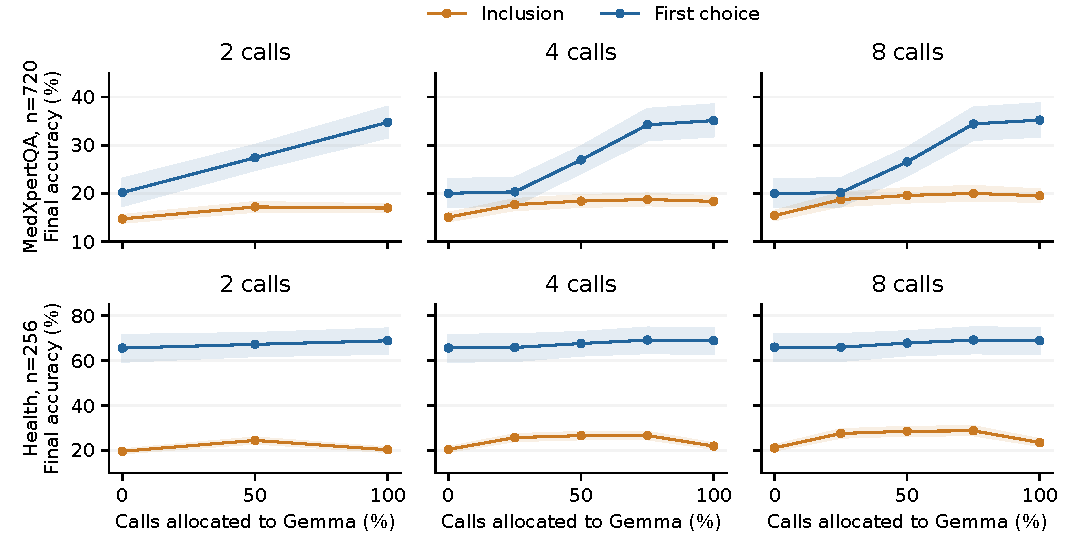
\includegraphics[width=\linewidth]{figures/ALLOCATION_BUDGET.pdf}
\caption{Exploratory allocation--budget sensitivity: 720 native and 256 Health questions. Points average stored-call subsets and banks, including at eight calls; they are not the primary fixed-slot estimates. Lines connect feasible allocations, not continuous policies. Shading: pointwise 95\% question-bootstrap intervals, not adjusted $C$ intervals. Call budgets are matched. Five rules are evaluated; inclusion and first-choice curves are shown.}
\label{fig:allocation_budget}
\end{figure}
\begin{table}[t]
\centering\small
\caption{Balanced-mixture $C$ across call budgets (percentage points), from the exploratory finite-bank replay in Figure~\ref{fig:allocation_budget}. Adjusted intervals cover the six source--budget contrasts using whole-question resampling. All questions were previously inspected; no fixed-slot primary is replaced.}
\label{tab:allocation_budget}
\begin{tabular}{llrrr}
\toprule
Source & Calls & $C$ & Pointwise 95\% & Adjusted six\\
\midrule
MedXpertQA &2&7.59&[6.05,9.12]&[5.50,9.64]\\
&4&8.23&[6.46,10.02]&[5.84,10.59]\\
&8&8.76&[6.62,10.92]&[5.85,11.63]\\
Health &2&5.76&[3.11,8.43]&[2.16,9.36]\\
&4&5.89&[2.99,8.80]&[1.96,9.78]\\
&8&6.10&[2.93,9.28]&[1.85,10.36]\\
\bottomrule
\end{tabular}
\end{table}
\subsection{Partner-composition sensitivity on recorded ballots}\label{app:partner_composition}

This exploratory replay reuses all 288 Native288 questions and their two banks, rather than generating new responses. Each bank contains eight Gemma calls and two calls each from Llama8B, Ministral14B and Qwen14B. At a four-call budget, H4 averages all $\binom{8}{4}=70$ Gemma subsets. For each partner, M2+2 averages all $\binom{8}{2}=28$ Gemma subsets combined with that partner's two stored calls. All five rules and uniform final ties are retained; failed calls remain empty. Subsets are averaged within bank, then banks within question. This estimates a finite recorded-list policy, not performance over independently resampled model outputs.

The original eight-call primary point estimate and every original absolute rule accuracy are reconstructed before the new calculation. An independently written exact-Fraction scorer checks 1,732 mixtures and edge cases against the integer implementation. Fifty thousand whole-question bootstrap draws, stratified by the three native tasks, preserve dependence across partners, rules, subsets and banks. The family consists of $C$, the inclusion allocation difference and the first-choice allocation difference for each of three partners: nine contrasts, with Bonferroni percentile tail probability $.05/18$. Intervals are nominal bootstrap intervals, not finite-sample coverage guarantees. All comparisons are exploratory; none replaces the original primary or selects a new policy.

\begin{table}[h]
\centering\small
\caption{Four-call partner replay on Native288. Accuracy is percent; differences and adjusted intervals are percentage points. H4 inclusion/first-choice accuracies are 17.55/29.86. All intervals adjust over the nine contrasts.}
\label{tab:partner_composition}
\begin{tabular}{lrrrr}
\toprule
Partner & M inclusion & M first & $C$ [adjusted 95\%] & First M--H [adjusted 95\%]\\
\midrule
Llama8B &16.08&24.30&$4.08\ [.21,8.07]$&$-5.56\ [-8.99,-2.10]$\\
Ministral14B &18.39&23.26&$7.43\ [3.09,11.87]$&$-6.59\ [-10.78,-2.36]$\\
Qwen14B &16.40&22.84&$5.86\ [1.62,10.17]$&$-7.01\ [-11.34,-2.74]$\\
\bottomrule
\end{tabular}
\end{table}

The inclusion allocation differences are $-1.48\ [-4.18,1.27]$, $.84\ [-1.18,2.86]$ and $-1.15\ [-3.36,1.02]$ points in the same order. Positive $C$ therefore remains distinct from a demonstrated mixed-policy gain. The three comparisons share cases and a Gemma reference, differ in partner quality, and change the original eight-call allocation. They broaden the descriptive composition check without establishing independent replication, a model-size law or quality-independent lineage causality. The separate composition replay includes the stripped ballots, task/answer keys, case vectors, all five-rule accuracies, bank means and bootstrap seed 202609160044.

\section{Prediction and secondary selector comparisons}\label{app:readability_detail}

The held-out predictor tests whether observed tie incidence predicts question-level rule effects. Define $c_i$ by inserting question $i$'s bank-averaged scores into Eq.~\ref{eq:C}; $C$ is the mean of $c_i$. Ridge regressions train on the earlier 128 native cases and predict $c_i$ on Native288. The two baseline features are the M-minus-H differences in distinct candidate count divided by ten and in maximum first-choice count divided by eight. The extension adds H-minus-M inclusion-tie indicators. Features average banks, are training-standardized and use unit ridge penalty. Mean squared error (MSE) uses squared-proportion units. Held-out MSE reduction (baseline minus extended) is effectively zero: $0.0000003\ [-.00290,.00296]$ (95\% interval; Appendix~\ref{app:representation}); positive reduction favors the tie feature. Both models were frozen after generation began but before fresh accuracy analysis. Explaining vote arithmetic has not yielded a useful new-case predictor.

For the separate Native720 quality/lift decomposition, the paired components have bootstrap covariance $0.126$ points$^2$, and bank-level lift differences are $-1.58/-1.71$ points. These descriptive quantities do not establish quality-independent causality.

Under shared uniform tie-breaking priority, Native720 $H_G$ first-choice has expected correction and reversal rates of 24.37\% and 8.64\% relative to inclusion, averaging banks. Question-level $C$ is positive/zero/negative on 305/285/130 native questions and 143/67/46 Health questions. Inclusion obscures a correct unanimous homogeneous first choice in at least one bank on 184/720 and 166/256 questions, respectively. These are retrospective output-defined counts, not prospective predictors.

\subsection{Secondary selector interventions and estimands}\label{app:selector_detail}

Two secondary tests examine LLM selectors: shuffle support numbers within each allocation's pool, or reverse support ranks in a common pool. These are different interventions, not replications.

The \emph{support-number test} uses each allocation's own pool. Selectors read the case, rationales, inclusion counts and reciprocal-rank sums. TRUE supplies actual support; SHUFFLED reassigns support pairs, keeping candidates fixed within allocation. For example, $(6,4)$ for A and $(2,1)$ for B becomes $(2,1)$ for A and $(6,4)$ for B.

For a selector or voting rule $s$, define $D_s=(F_{M,\mathrm{TRUE}}-F_{M,\mathrm{SHUFFLED}})-(F_{H,\mathrm{TRUE}}-F_{H,\mathrm{SHUFFLED}})$. It measures whether correct support helps M more than H. We then compare the LLM with voting: $J=D_{\mathrm{LLM}}-D_{\mathrm{vote}}$. A negative $J$ need not mean support harms the LLM. If correct support helps its M decisions by two points and H by six, $D_{\mathrm{LLM}}=-4$; if voting gains one point in each, $D_{\mathrm{vote}}=0$ and $J=-4$. These illustrative numbers explain the contrast, not the observed effect.

On 96 MedEinst pairs, Gemini's $J=-16.54\ [-27.30,-6.47]$ and Llama's $-13.41\ [-23.35,-3.95]$ points (97.5\% intervals). Using tie-aware inclusion---RR only for ties---instead shifts both by 11.33 points: $-5.21\ [-14.58,4.17]$ and $-2.08\ [-10.94,6.77]$ (exploratory 95\% intervals). No LLM output changes: the reference, not an internal mechanism, changed.

Neither negative contrast reproduces on 128 native-key questions. Here mixed pools more often contain a correct key: the availability gain is 6.25 points $[2.34,10.94]$. Neither selector chooses any of the eight keys available only in mixed pools. Availability therefore need not be converted into a correct decision \citep{chen2026routinggap}. Source and answer format change together, preventing separate attribution. These findings are supporting boundaries, not confirmation of $C$ or $\theta$.

The \emph{support-rank test} compares LLM and top-rank selection from a pool shared across allocations. On 224 reused cases, that pool is the H/M union for MedEinst and all native options. Inclusion count, then RR, then a deterministic hash give unique ranks. Selectors see ranks in forward or reversed order instead of counts. Here $D$ is M-minus-H in the forward-minus-reversed accuracy change; $J_{\rm norm}=D_{\mathrm{LLM}}-D_{\mathrm{top\ rank}}$ compares selectors. This changed intervention and reference cannot confirm $J$. Only Llama on MedEinst has a positive 98.75\% interval, $8.85\ [3.13,15.10]$ percentage points; the other three include zero. The positive interaction partly reflects weaker mixed rankings, not better mixed selection.

\section{Local reproduction, resources and access}\label{app:repro}

\paragraph{Portable saved-output replay.}
Extract the separate \path{representation_replay.zip}, install NumPy, and run \texttt{python3 replay.py} from the extracted directory. The entry point verifies input checksums and runs eight checks: representation/mapping sensitivity, the 720-question decision analysis, quality/lift accounting, the empirical-list reference, Health transport, the answer-contract test, development-selected joint policies, and allocation/budget curves. Inputs are scored ranks and case identifiers; outputs are reconstructed rule scores, contrasts and uncertainty checks. This requires no model access or credentials. It replays stored-output inference, not fresh hosted sampling or clinical adjudication. Question text and full provider payloads are not included. The separate manuscript-source archive builds the PDF with \texttt{latexmk -pdf main.tex}; it is not an inference runner.

\paragraph{Serving and repair details.}
\textit{Answer-key access by stage.} Development labels select policies; generators receive questions/options or patient records, not answer keys. Secondary LLM selectors receive candidate text, rationales and support without the key. Voting and rank-transfer operators form decisions without it; scoring then uses it. Retries respond to service/parsing failure, not correctness. Gold-informed membership ceilings, wrong-answer relabeling and hindsight routing use held-out keys for diagnosis, so they are not label-free deployable policies. Changing key metadata leaves all 31,232 scheduled Native720/Health generation messages unchanged. This checks prompt construction, not pretraining contamination or independent clinical validity.

Of 192 Qwen generator identities, 27 came from hosted Featherless inference and 165 from a RunPod/vLLM fallback using the named official 14B weights. Gemma requests were routed among eight serving providers; the nominal endpoint does not fix their kernels or quantization. The original automated mapping used \path{google/gemma-3-12b-it} and \path{microsoft/phi-4}; the seven-cell local repair used \path{Qwen/Qwen2.5-1.5B-Instruct}, a different model from the generator. Three natural-selector formatting repairs preserved top-one identities. C3B ran on 6 September 2026 and returned Google as provider for all 576 choices. C2 cost \$0.244793. The C3/C3B interface experiments used 1,157 requests including five identical retries. The subsequent scoring and rule replays added no inference cost. These implementation qualifications do not establish clinical adjudication or equivalent remote serving implementations.

The manuscript-source archive contains text, official styles, bibliography and figures/tables, not a public experimental dataset. Stored-output replay is distinct from hosted regeneration and terminology adjudication. Original traces and scoring corrections remain archived; credentials are excluded.

\subsection{Replay resources and notation}\label{app:reader_card}

The accompanying \path{ballot_diagnostics_v1.zip} contains 31,232 scheduled native-key lists across 976 questions and two banks, a versioned schema/data card, executable analyses, expected results and checksums. Terminal failures are empty lists. It supports new rule evaluation without regenerating model answers, but is a local anonymous submission artifact, not a public DOI deposit. Install Python and NumPy; run \texttt{python3 replay.py --data data --out outputs}, then \texttt{python3 null.py --data data --out outputs}. Compare the three JSON outputs with \path{expected/}. These commands need no network, question text, model credentials, or clinical dictionaries.

\paragraph{Notation and interval guide.}
$C$ is the inclusion-minus-first allocation interaction; $C_G$ names the same contrast against Gemma on Health. $\theta$ is mixed-minus-selected-Gemma first-choice accuracy. $\Delta q$ is the per-call accuracy difference; $\Delta L$ is the difference in aggregation lift, an accounting quantity. $R=\theta_{K5}-\theta_{K1}$ compares answer contracts. $v$, $s$ and $\beta$ denote availability, conditional selection success and pool co-failure. Original sole primaries have pointwise 95\% intervals. Rank randomization uses eight adjusted endpoints; transfer four; IRV six; task breakdown six; partner replay nine; policy comparisons 28. The secondary selector quantities are defined in Section~\ref{app:selector_detail}: $D$ is the support-intervention interaction, $J$ subtracts a voting reference, $J_{\rm norm}$ uses a different support-rank intervention and reference, and $\Delta_A$ is an availability difference. The two-selector $J$ family uses 97.5\% marginal intervals; four-cell common-pool intervals are 98.75\%. Exploratory reference changes use the interval level stated at their result.

\paragraph{Cost and serving limits.}
Dividing Native720 H's recorded eight-call resources by eight gives a uniformly sampled single-slot reference of 585.9 input and 149.1 output tokens, approximately \$0.000098 per question, and 34.48\% accuracy. This uses the same five-answer contract and includes recorded retry costs; it is not a newly run direct-answer model. Batch durations (e.g. Health 1,432 seconds) combine concurrent dispatch and retries and do not identify deployment request latency. The retained logs identify named endpoints/providers and request dates, but do not supply exact weight snapshots for all hosted calls. Missing snapshot hashes remain unknown; open-weight model names do not certify local serving equivalence.

\section{Mapping correction and construct scenarios}\label{app:mapping}
The versioned union consists of 4,510 earlier A0 pairs and 1,770 C2 pairs with 812 overlap. Version 3 repairs five relations globally: three Ebola disease synonyms, the explicit non-Ebola exclusion, and Koch's disease as a tuberculosis synonym. Version 4 repairs 35 further relationships using source-backed text rules. Strict labels are unchanged from v3. The complete change ledgers include reference/candidate strings, old and new relations, rule identifiers and source locators. Their scope includes the full C1 inventory, not just outcome-relevant C2 cases.

NLM distinguishes a MeSH Concept's synonym group from its broader Descriptor: \url{https://www.nlm.nih.gov/mesh/concept_structure.html}. The correction uses ConceptUI identity, verified aliases/acronyms and target-negation checks. CDC pharyngitis guidance distinguishes streptococcal from viral disease: \url{https://www.cdc.gov/group-a-strep/hcp/clinical-guidance/strep-throat.html}. CDC respiratory guidance distinguishes upper-airway diagnoses from bronchitis/pneumonia: \url{https://www.cdc.gov/antibiotic-use/hcp/clinical-care/adult-outpatient.html}. ACS includes both infarction and unstable angina: \url{https://medlineplus.gov/ency/article/007639.htm}. The complete source index is local; source reading is not case adjudication.

The source-coded audit links all 49 released targets to the official CDC FY2026 order file, retaining the source's undeclared coding vintage as a limitation. For example, Bronchitis has unspecified J40, pulmonary/pancreatic neoplasm names omit the malignancy in C34/C25, and Pericarditis omits the acute state in I30. Other code/name mismatches include the broader asthma code for a compound acute-episode target. Codes never silently override the primary map.

Temporal modifiers are acute, chronic, recurrent, recurrence and exacerbation; etiologic modifiers are viral and bacterial; severity/site modifiers are severe, mild, left, right and bilateral. Only candidate modifiers absent from the full reference can be removed, and the remainder must match the full reference through independent synonym rules. This recognizes 18 temporal, ten etiologic and two severity/site pair incidences (classes can overlap). All eight subsets are evaluated. A separate finite source-coded sensitivity concerns explicit terms for pulmonary/pancreatic malignancy, acute pericarditis and myocardial infarction. It affects eight inventory pairs; it is not an exhaustive clinical scoring system.

The 14 priority source dispositions agree with the final map. All 106 original class controls are retained; 675 C2 relations remain flagged unresolved. Regression checks cover historical/current mentions, contradictory etiology, upper/lower disease, episode specificity, alternatives, negation, causal clauses and unverified parentheses. Broad v3 mapper-disagreement extrema remain preserved as stress bounds, not clinically plausible confidence bounds; the present scenarios provide narrower, source-motivated construct checks without claiming exhaustive semantic coverage.

\section{Secondary study protocols and development limitations}\label{app:support_screens}
These studies ask whether a selector uses the candidate support supplied by generators. The intervention changes the displayed support while retaining each candidate pool. The direct interaction $D$ compares the effect on mixed and homogeneous pools; $J$ subtracts that interaction for a specified voting rule (Section~\ref{app:selector_detail}). A negative $J$ therefore concerns the LLM relative to that reference, not necessarily an absolute loss in LLM accuracy. The development, MedEinst confirmation and native-key transport below use different cases and must remain separate.

In the 128-question native-key support transport, Gemma's per-call first-choice accuracy is 305/1,024, versus 31/256, 33/256 and 32/256 for the other generators. These descriptive quality differences accompany the larger mixed candidate pools; they do not identify a quality-independent lineage effect.

On 48 development pairs, the original positive rescue fails: Gemini's refinement interaction is $-.0625$ (95\% CI $[-.1562,.0312]$), with strict $+.0104$ $[-.0833,.1042]$. Exploratory frequency-relative $J$ is $-.1840$ $[-.2969,-.0790]$ strict and $-.2309$ $[-.3394,-.1276]$ with refinements.

\subsection{Earlier native support-study cells}\label{app:earlier_native_cells}
Table~\ref{tab:medx} preserves the full earlier 128-item support-intervention cells. It is a different cohort and estimand from the fresh 288-item representation primary. Section~\ref{sec:support_boundaries} reports the unresolved transport and available-but-unselected keys.

The correct key is available on 114 H and 122 M questions, while the best deterministic rule scores 38 expected correct H selections. Availability is therefore much larger than achieved voting accuracy on this earlier cohort; these are not the Native720 pools.

\begin{table}[htbp]
\centering\small
\caption{Earlier MedXpertQA support study: expected correct selections out of 128 native-key questions. Fractional cells integrate uniform ties for deterministic rules; LLM rows count actual correct choices. Same support interface; no clinical semantic judge.}
\label{tab:medx}
\begin{tabular}{lrrrr}
\toprule
Rule & H TRUE & H SHUFFLED & M TRUE & M SHUFFLED\\
\midrule
Gemini &42&27&29&23\\
Llama 8B &32&24&28&15\\
Inclusion frequency &23.98&15.98&22.08&10.75\\
First choice &37.50&14.00&21.42&11.42\\
Frequency + RR ties &37.00&13.50&22.00&14.50\\
Reciprocal rank &37.50&13.50&23.00&13.33\\
Borda &38.00&13.50&22.50&15.50\\
Oracle &114&114&122&122\\
\bottomrule
\end{tabular}
\end{table}

\subsection{Earlier development design}\label{app:pipeline}
The earlier 48-pair MedEinst study motivated, but does not independently confirm, the native-key studies. An outcome-blind hash-ranked selection balanced transition frequency and narrative length into 16/16/16 strata. Its 96 branches are correlated pairs, not independent cases. The separate 36-case DDXPlus boundary already had a correct concept in every pool under both policies and cannot show increased availability or independent clinical transport. Full early screening records remain in the archival version; material scoring and failure qualifications follow.

\subsection{Diagnostic generation and selection}\label{app:prompts}
Each branch uses eight Gemma calls and two each from Llama, Ministral and Qwen; the mixed allocation reuses two Gemma calls. The generator system message was:
\begin{quote}\footnotesize\ttfamily
You are performing a controlled diagnostic benchmark. Use only the supplied patient record and return the requested JSON.
\end{quote}
The user template was:
\begin{quote}\footnotesize\ttfamily
Generate a ranked differential diagnosis using only this patient record. Return exactly five distinct plausible diagnosis names, ordered most to least likely. For each, give one evidence-linked rationale of at most 18 words. Do not assume a supplied candidate list, another case version, or other agents.

Patient record:\\
\mbox{[PATIENT\_RECORD]}

Return only one JSON object:\\ \{"candidates":[\{"diagnosis":"name", "rationale":"at most 18 words"\}, ... exactly five items]\}. Do not use markdown fences or add keys.
\end{quote}
Generation uses temperature 1, top-$p=.9$ and 384 output tokens. All 1,344 scheduled proposals are included. Qwen contributes 27 hosted and 165 local responses after 59 provider failures; one malformed local output receives the allowed same-prompt retry. These serving implementations are not established equivalent (Section~\ref{app:repro}).

The natural selector, Gemini2.5-Flash-Lite, receives the patient record, opaque candidate IDs, diagnosis text and one representative rationale. Source, frequency and allocation labels are withheld; candidate order is hash-derived. It returns a complete ID permutation at temperature 0, top-$p=1$, maximum 300 tokens. All 192 canonical rankings are valid after 198 raw attempts; three format-only repairs preserve the original top choice. No failed identity is dropped. The earlier mapping uses Gemma3-12B and Phi4 at temperature 0, top-$p=1$, maximum 5,000 tokens. Diagnosis-only pairs receive one of four relations: synonym, parent/subtype, compound/context-dependent, or non-equivalent. Of 1,916 novel mapping cells, 1,909 come from the provider and seven are completed locally before analysis. Neither model agreement nor this repair is clinical adjudication.

\subsection{Development scoring and failed tests}\label{app:statistics}\label{app:results}\label{app:interface}
Natural-effect intervals resample whole case pairs 50,000 times (seed 20260905185214). Scoring corrections are retrospective: investigators had seen aggregate results. Rules apply globally to diagnosis pairs, and intervals condition on the chosen map rather than jointly accounting for semantic uncertainty. Frequency counts distinct proposing calls; reciprocal rank uses the best occurrence in each call. Uniform ties and ambiguous surface representatives receive expected correctness, never any-member credit. These rules see support information withheld from the natural selector.

Strict availability is 51/96 versus 60/96 for H/M, with 18/96 versus 10/96 final correct choices. Crediting temporal and other whitelisted refinements changes availability to 60/96 versus 62/96 and final choices to 20/96 versus 14/96. Eight apparent mixed-only opportunities disappear because H's ``Acute Bronchitis'' receives credit against ``Bronchitis.'' Thus these outputs do not establish robust clinical-concept complementarity. No strict mixed-only opportunity converts; one of three refinement opportunities does. Section~\ref{app:mapping} retains the correction authority and unresolved-label limits.

The candidate-set-size test uses 11 mixed-only branches matched to 11 both-available controls by a pre-output difficulty instrument, two sizes ($k=2,8$) and two orders: 88 valid rankings. Original and corrected-strict ten-match intervals include zero. Temporal credit leaves only two eligible matches with identical observed interactions, yielding a degenerate empirical interval $.5\ [.5,.5]$; that is not evidence of a general competition mechanism. An additional refinement-eligible branch has no saved intervention and is not imputed.

The metadata screen changes only supplied support counts/ranks within each pool: hidden, true, or cyclically reassigned metadata. All 576 fresh single-ID choices use Gemini2.5-Flash-Lite at temperature 0, top-$p=1$, maximum 64 tokens and a shared per-pool seed. It fails its prespecified positive-rescue criterion: interaction at least .05, positive 97.5\% case-pair-bootstrap lower limits for both the interaction and mixed true-minus-shuffled contrast, and positive strict-score directions. Historical full rankings are not its control arm. Its preceding full-ranking attempt produced 571/576 valid outputs after 581 attempts and was not scored; the uniform single-ID repair preceded accuracy inspection, and no predecessor outputs were pooled. Negative estimates and later, distinct selector tests remain in Section~\ref{app:support_screens}. These synthetic benchmark studies do not establish patient benefit.

\section{Further tests of information loss and decision value}\label{app:review_followthrough}
These analyses address different limits of the central comparison. They reuse stored answers and are exploratory; they add neither cases nor independent confirmation. Native288 uses its original four-model allocation. Native720 and Health256 use eight Gemma calls, eight Llama3.3-70B calls and the first four scheduled slots from each. Empty failed slots remain. Except for the explicitly labeled Monte Carlo reference distributions, intervals resample whole questions, average banks, and retain native task strata. A common 20,000-draw bootstrap (seed 20260921) supplies nominal intervals and the family adjustments specified below. The original primary intervals, obtained with their own frozen seeds and 50,000 draws, remain authoritative.

\subsection{Prespecified endpoints and generation failures}
The representation study froze native $C$ before new generation; MedEinst was a prespecified secondary transport with uncertain mappings. The 720-question study froze first-choice $\theta$ after development-only selection among ten homogeneous policies. Health froze $C_G$ before its generations. The later fifteen-policy search was specified after test outcomes were known, but selected its winner using development data only. K1/K5 generated fresh answers on 128 new questions under a separately frozen contract comparison; its unresolved primary missed the precision target. Depth, budget, partner, rank-transfer, information-bound, relabeling, screening and oracle results are saved-output analyses, not additional replications. The held-out predictor's recipe was frozen after generation began but before fresh accuracy analysis.

The original attempt audit reconciles 13,440 slots with 13,845 attempts, first-valid retention and at most one identical-payload retry. Every source/model cell passes the protocol's terminal-failure threshold of at most 5\% (Table~\ref{tab:failure_cells}). A failed first attempt followed by success is an attempted retry, not a terminal failed slot. Meeting this failure threshold does not resolve scoring or scientific transport uncertainty.

\begin{table}[ht]
\centering\small
\caption{Original representation study: scheduled slots, actual attempts including retries, terminal failures and percentage of scheduled slots failing. All eight source/model cells are below the prespecified 5\% failure limit.}
\label{tab:failure_cells}
\begin{tabular}{llrrrr}
\toprule
Source & Model & Slots & Attempts & Failures & \%\\
\midrule
medeinst & gemma & 3072 & 3104 & 5 & 0.16\\
medeinst & llama & 768 & 788 & 0 & 0.00\\
medeinst & ministral & 768 & 773 & 2 & 0.26\\
medeinst & qwen & 768 & 771 & 1 & 0.13\\
native & gemma & 4608 & 4863 & 85 & 1.84\\
native & llama & 1152 & 1218 & 43 & 3.73\\
native & ministral & 1152 & 1153 & 0 & 0.00\\
native & qwen & 1152 & 1175 & 12 & 1.04\\
\bottomrule
\end{tabular}
\end{table}

\subsection{Tie accounting and rule-eligible selection}
For each question, define $T=(F_{H,\mathrm{tie}}-F_{H,\mathrm{incl}})-(F_{M,\mathrm{tie}}-F_{M,\mathrm{incl}})$ and $U=(F_{M,\mathrm{tie}}-F_{H,\mathrm{tie}})-(F_{M,\mathrm{first}}-F_{H,\mathrm{first}})$. Then $C=T+U$ exactly before and after averaging. Six component endpoints (three cohorts, $T/U$) share a Bonferroni family. The unresolved remainders do not establish equivalence. Conditioning on observed masking is descriptive: the contribution from questions with at least one correct unanimous H first-choice bank masked by an inclusion tie is calculated using the full cohort denominator, not as a subgroup average.

\begin{table}[ht]
\centering\small
\caption{Paired decomposition in percentage points. T/U intervals adjust across six components. Masked and other contributions sum to C; their columns are point estimates using the full question denominator.}
\begin{tabular}{lrrrr}
\toprule
Cohort & T [adjusted 95\%] & U [adjusted 95\%] & Masked & Other\\
\midrule
Native288 & $7.62\ [2.04,13.32]$ & $2.10\ [-1.85,6.11]$ & 6.90 & 2.82\\
Native720 & $8.73\ [5.48,11.95]$ & $0.45\ [-1.86,2.81]$ & 6.42 & 2.76\\
Health256 & $5.98\ [1.25,10.52]$ & $0.16\ [-2.80,3.19]$ & 9.06 & -2.92\\
\bottomrule
\end{tabular}
\end{table}

First-choice eligibility means that gold appears at rank one in at least one selected list. All-rank availability means it appears anywhere. We calculate conditional success as pooled final accuracy divided by pooled eligibility, recomputing both terms in each bootstrap. For first-choice voting, the error decomposes as $1-F=(1-v_1)+(v_1-F)$: inaccessible gold plus failure despite rank-one access. The denominator is the full set of scheduled questions and banks, including failures. The archive additionally reports minimum-gold-rank frequencies (ranks one to five, or absent), all-rank conditional success, and paired intervals.

The exact counts make the conditioning explicit. Native720 has 1,440 question--bank records: H/M have gold at any rank in 1,291/1,327 records and at rank one somewhere in 671/709. Their expected correct totals are $6085/12$ and $2269/6$, yielding $100(6085/12)/671=75.57\%$ and $100(2269/6)/709=53.34\%$ conditional success. Health has 512 records: all-rank counts 493/501, rank-one counts 380/411, and expected correct totals $1057/3$ and $693/2$, yielding 92.72/84.31\%. These fractional totals average uniform voting ties; they are not counts of independently observed successes. Resampling keeps both banks together within each question. Comparing conditional rates on different eligible sets is descriptive, not a matched intervention on selector ability.

\begin{table}[ht]
\centering\small
\caption{Eligibility and selection (percent). F/v1 uses pooled values; it is not an average of question-level ratios.}
\begin{tabular}{llrrrrr}
\toprule
Cohort & Policy & Rank-one v1 & All-rank v & F/v1 & Inaccessible & Eligible error\\
\midrule
Native288 & H & 43.75 & 86.28 & 68.25 & 56.25 & 13.89\\
Native288 & M & 50.17 & 89.58 & 37.69 & 49.83 & 31.26\\
Native720 & H & 46.60 & 89.65 & 75.57 & 53.40 & 11.38\\
Native720 & M & 49.24 & 92.15 & 53.34 & 50.76 & 22.97\\
Health256 & H & 74.22 & 96.29 & 92.72 & 25.78 & 5.40\\
Health256 & M & 80.27 & 97.85 & 84.31 & 19.73 & 12.60\\
\bottomrule
\end{tabular}
\end{table}

\begin{table}[ht]
\centering\small
\caption{Eight-call first-choice minus a uniformly selected scheduled single slot, using the same five-answer contract. Intervals adjust over four contrasts; neither interval type is evidence of equivalence.}
\begin{tabular}{llrr}
\toprule
Cohort & Policy & Gain [95\%] & Gain [adjusted 95\%]\\
\midrule
Native720 & H & $0.73\ [-0.01,1.49]$ & $0.73\ [-0.19,1.69]$\\
Native720 & M & $-0.91\ [-1.82,0.03]$ & $-0.91\ [-2.07,0.27]$\\
Health256 & H & $0.09\ [-0.66,0.82]$ & $0.09\ [-0.86,1.01]$\\
Health256 & M & $1.10\ [0.10,2.12]$ & $1.10\ [-0.15,2.42]$\\
\bottomrule
\end{tabular}
\end{table}

MedEinst requires a separate scoring qualification. We recompute the tie remainder under the implemented refinement criterion, a protocol-consistent sensitivity zeroing new unresolved relations, and strict synonyms. Nominal intervals condition on each fixed map; three adjusted remainder intervals cover these sensitivities. Negative values remain properties of those maps, not clinical counterexamples to the native-key decomposition.

\begin{table}[ht]
\centering\small
\caption{MedEinst mapping-conditional C, T and U in points. No terminology adjudication is added.}
\begin{tabular}{lrrr}
\toprule
Scoring & C & T & U [adjusted 95\%]\\
\midrule
protocol\_consistent & 4.93 & 11.69 & $-6.76\ [-11.59,-2.01]$\\
refinement & 4.85 & 11.69 & $-6.85\ [-11.67,-2.06]$\\
strict & 6.10 & 11.67 & $-5.57\ [-10.20,-1.01]$\\
\bottomrule
\end{tabular}
\end{table}

\subsection{A ceiling for selectors without ranks}
A candidate-name-neutral selector is equivariant: renaming candidates in its input merely renames its output distribution. Assume it sees no question text, rationale, semantic candidate attributes or answer key, and can select only candidates appearing in the pool. One representation supplies each candidate's total inclusion count. A richer representation supplies the entire binary candidate-by-call matrix, retaining call order and therefore model membership, but omitting ranks.

For the count representation, place candidates with the same count in one class. For the matrix, place candidates with identical rows of call membership in one class (equivalently, identical columns if candidates index columns). If the gold candidate belongs to a class of size $k$, its selection probability is at most $1/k$; if absent it is zero. To see why, swap gold with any candidate in its class. The represented input is unchanged, while equivariance swaps their output probabilities. All $k$ probabilities must therefore be equal and sum to at most one. Averaging the per-pool bound gives a ceiling on mean accuracy for every selector in this restricted class. This elementary symmetry argument is not a new general decision theorem.

The argument conditions on each realized pool: it assumes neither independent errors nor equal generator accuracy. The ceiling uses gold to identify its class, so it need not be attainable: a real selector also has to choose the right class. It permits arbitrary use of model-specific membership patterns. It does not cover a semantic judge, rationale reader or a rule exploiting the original answer-letter positions. Ranked voting lies outside the restricted class because exchanging identical membership columns need not preserve ranks. A positive paired gap shows information available in ranks beyond this representation; a negative gap does not show that membership suffices for an attainable selector.

\begin{table}[ht]
\centering\small
\caption{First-choice accuracy versus gold-informed symmetry ceilings (percent), and its gap above the stronger full-membership ceiling (points). Gap intervals adjust over eight source/allocation/representation contrasts; the count-gap endpoints are retained in the archive.}
\begin{tabular}{llrrrr}
\toprule
Cohort & Policy & Count ceiling & Full membership & First choice & Gap [adjusted 95\%]\\
\midrule
Native720 & H & 39.68 & 44.21 & 35.21 & $-8.99\ [-15.18,-2.92]$\\
Native720 & M & 44.98 & 53.72 & 26.26 & $-27.46\ [-33.04,-21.95]$\\
Health256 & H & 28.59 & 30.28 & 68.82 & $38.54\ [28.86,47.46]$\\
Health256 & M & 35.65 & 38.42 & 67.68 & $29.25\ [19.84,37.83]$\\
\bottomrule
\end{tabular}
\end{table}

\subsection{Changing wrong-answer alignment at fixed correctness}
For every question and model, sample a uniform bijection over the nine incorrect option IDs, fixing gold. Reuse it for every list of that model in both banks. Different models receive independent permutations. This preserves each correct answer's rank or absence, every failure, and all within-model equality relations. The mixed allocation reuses the same transformed Gemma slots as H. Unlike shuffling lists across questions, this operation also preserves the entire question-by-call correctness matrix and question difficulty alignment.

All homogeneous scores must be unchanged for every draw and rule. Applying one common candidate permutation to both models must also preserve every mixed score; both controls pass. Model-specific permutations change wrong-answer agreement without changing per-call accuracy. They do not preserve candidate meanings and use the gold key, so they cannot be supplied to a semantic judge or deployed as an improvement. There is no claim about counterfactually retrained models.

We use 256 draws (seed 20260994). The archive reports each rule's mixed accuracy change, changes in rule-versus-first interactions, randomization reference ranges, changed-outcome frequency and split-half Monte Carlo checks. Question-bootstrap intervals condition on the per-question simulation means; permutation ranges describe the randomization distribution and are not confidence intervals. Ten rule-interaction changes across two sources form a family (the first-versus-itself contrast is identically zero). Separate ten-endpoint adjustment covers the five mixed-accuracy changes per source.

\begin{table}[ht]
\centering\small
\caption{Synthetic wrong-option alignment: changes in mixed accuracy and the rule-versus-first interaction, in points. The original H scores are invariant. Intervals adjust within the respective ten-endpoint families.}
\begin{tabular}{llrr}
\toprule
Source & Rule & Mixed accuracy change & Interaction change\\
\midrule
Native720 & inclusion & $11.29\ [9.95,12.64]$ & $11.08\ [9.74,12.44]$\\
Native720 & first & $0.21\ [-0.01,0.51]$ & $0.00\ [0.00,0.00]$\\
Native720 & tie & $13.72\ [11.25,16.28]$ & $13.51\ [11.07,16.04]$\\
Native720 & rr & $9.26\ [7.05,11.63]$ & $9.05\ [6.88,11.35]$\\
Native720 & borda & $14.90\ [12.17,17.74]$ & $14.68\ [12.01,17.47]$\\
Health256 & inclusion & $15.56\ [13.58,17.40]$ & $15.52\ [13.55,17.37]$\\
Health256 & first & $0.04\ [0.00,0.19]$ & $0.00\ [0.00,0.00]$\\
Health256 & tie & $8.91\ [5.61,12.63]$ & $8.88\ [5.59,12.54]$\\
Health256 & rr & $6.70\ [3.54,10.34]$ & $6.66\ [3.52,10.30]$\\
Health256 & borda & $10.91\ [6.73,15.55]$ & $10.88\ [6.70,15.53]$\\
\bottomrule
\end{tabular}
\end{table}

Native720: 49.90\% of bank-level mixed outcomes change in at least one rule, averaged over draws. The randomization 95\% range for the change in $C$ is $[9.98,12.35]$ points. Monte Carlo standard error of its population mean is 0.04 points. The maximum population-mean difference across the two draw halves is 0.116 points across five mixed-rule accuracies. Individual-question means are less precise; no interpretation treats simulation draws as independent questions.

Health256: 71.80\% of bank-level mixed outcomes change in at least one rule, averaged over draws. The randomization 95\% range for the change in $C$ is $[13.54,17.70]$ points. Monte Carlo standard error of its population mean is 0.07 points. The maximum population-mean difference across the two draw halves is 0.052 points across five mixed-rule accuracies. Individual-question means are less precise; no interpretation treats simulation draws as independent questions.

\subsection{Donor ranks, reusable headroom and equal-budget screening}
\label{app:budget_donor}
The neutral donor sensitivity replaces deterministic SHA ordering of equal donor scores with one uniformly random candidate priority shared across the recipient's lists. Only the earliest donor-present position can affect that list's final first vote. An exact recursion averages the earliest member of the union of unresolved tied first-position candidates, resolves every affected list, and repeats; final vote ties still receive uniform credit. Exhaustive small examples agree with direct enumeration of candidate orders. Self and cross controls use the same operation. A frequency-only donor replaces reciprocal-rank scores by inclusion counts; direct donor-first accuracy provides the simple answer-import reference, without pretending to retain recipient memberships.

\begin{table}[ht]
\centering\small
\caption{Recipient accuracy after neutral-priority transfer (percent) and cross-minus-self (points). Each operator uses a separate four-contrast family. Cross-transfer uses twelve unique calls per bank; direct donor-first is a different procedure.}
\begin{tabular}{lllrrr}
\toprule
Source & Recipient & Donor score & Self & Cross & Change [adjusted 95\%]\\
\midrule
Native720 & H & rr & 34.65 & 25.57 & $-9.08\ [-12.34,-5.89]$\\
Native720 & H & frequency & 19.49 & 19.68 & $0.19\ [-1.28,1.63]$\\
Native720 & M & rr & 24.95 & 33.58 & $8.63\ [5.56,11.74]$\\
Native720 & M & frequency & 19.71 & 19.43 & $-0.29\ [-1.47,0.88]$\\
Health256 & H & rr & 69.04 & 68.46 & $-0.59\ [-4.88,3.61]$\\
Health256 & H & frequency & 23.48 & 28.55 & $5.07\ [3.35,6.94]$\\
Health256 & M & rr & 68.36 & 68.46 & $0.10\ [-4.20,4.49]$\\
Health256 & M & frequency & 28.48 & 25.09 & $-3.39\ [-5.05,-1.87]$\\
\bottomrule
\end{tabular}
\end{table}

The maximum absolute cohort-mean shift from replacing hash ties is .12 points on Native720 and .68 on Health; the full paired sensitivity intervals are archived. Direct donor-first yields the other allocation's original accuracy (26.26/35.21 on Native720 and 67.68/68.82 on Health for H/M recipients). Thus reranking does not establish superiority to simply using the strong donor. Frequency-only transfer has no resolved Native720 cross-minus-self effect, whereas neutral RR transfer retains both effects. Health's RR effects remain unresolved.

\paragraph{Eight-call donor allocation.}
Can donating ranks pay for the calls it consumes? We additionally freeze four allocations of eight stored calls: six Gemma proposals and two Llama donors, the reverse, four Gemma proposals and four Llama donors, and the reverse. Calls are the earliest scheduled slots, not selected successful or correct outputs. Donors reorder only candidates already in recipient lists, using the neutral-priority operator above. Ordinary first-choice, reciprocal-rank (RR) and Borda pooling use exactly the same eight outputs. Eight Gemma calls with first-choice voting remain the development-selected reference. Thus a gain over the recipient alone does not establish a useful allocation.

Table~\ref{tab:budget_donor} reports every allocation on the historically inspected Native720 and Health256 outputs. The two banks are averaged within question; 20,000 question bootstraps preserve original task strata. Five contrasts per allocation/source (three same-pool rules, Gemma eight-call reference and recipient-only first choice) form a 40-comparison exploratory family. Intervals condition on stored generations; they are not fresh confirmation. All contrasts and vectors are in the accompanying budget-transfer replay. Twenty-seven toy cases independently verify exact neutral-priority averaging.

\begin{table}[ht]
\centering\small
\caption{Fixed eight-call screen. A=Gemma, B=Llama; $6A+2B$ means six A recipient calls and two B donor calls. Accuracies are percent; the last column is transfer minus eight Gemma first-choice calls, with Bonferroni-40 bootstrap intervals in points. No allocation exceeds the reference's point estimate.}
\label{tab:budget_donor}
\begin{tabular}{llrrrrl}
\toprule
Source & Recipient+donor & Transfer & First & RR & Borda & Difference [adjusted 95\%]\\
\midrule
Native720 & $6A+2B$ &23.26&33.93&33.65&31.70&$-11.96\ [-16.88,-7.10]$\\
& $6B+2A$ &31.17&20.28&20.62&21.46&$-4.05\ [-7.38,-.80]$\\
& $4A+4B$ &23.23&26.26&24.86&25.06&$-11.98\ [-17.00,-7.05]$\\
& $4B+4A$ &32.40&26.26&24.86&25.06&$-2.82\ [-5.88,-.01]$\\
Health256 & $6A+2B$ &66.86&69.24&69.82&70.90&$-1.95\ [-9.96,6.05]$\\
& $6B+2A$ &67.29&66.11&66.02&68.55&$-1.53\ [-5.57,1.87]$\\
& $4A+4B$ &66.21&67.68&68.26&68.55&$-2.60\ [-10.66,5.47]$\\
& $4B+4A$ &66.60&67.68&68.26&68.55&$-2.21\ [-5.99,.65]$\\
\bottomrule
\end{tabular}
\end{table}

On Native720, $4B+4A$ gains 7.53 points $[3.83,11.35]$ over same-pool RR, but remains 2.82 points below eight Gemma calls. Stronger donor preferences can therefore improve weak recipient lists without beating a competent homogeneous policy. Health differences remain unresolved, not equivalent. The near-zero Native720 upper endpoint is sensitive to finite-bootstrap tail estimation and is not evidence for a general impossibility. This tests stored-generation donors, not fresh candidate-conditioned ranking calls or all possible allocations.

For cross-bank hindsight, select an optimal policy using the gold key and bank one, then evaluate that policy in bank two; reverse the roles and average. Uniformly average equally optimal selection policies. Compare against H first-choice in the same evaluation bank. The within-bank oracle uses the same candidate set and tie convention. The three candidate sets isolate allocation-only (three first-choice policies), rule-only (five H rules), and all fifteen policies. These label-using oracles measure repeated-output headroom on already known questions, not generalization to new questions or a realizable learned router. The previous oracle maximized after averaging banks; its different estimand cannot be subtracted to estimate noise.

\begin{table}[ht]
\centering\small
\caption{Hindsight gains above the unchanged H first-choice reference (points). Cross-bank intervals adjust over six contrasts. Within-bank results are point estimates under the same selection convention.}
\begin{tabular}{llrr}
\toprule
Source & Candidate policies & Within bank & Cross bank [adjusted 95\%]\\
\midrule
Native720 & allocation & 5.52 & $3.26\ [1.32,5.37]$\\
Native720 & rule & 9.63 & $6.18\ [4.64,7.70]$\\
Native720 & all & 18.26 & $12.11\ [9.73,14.57]$\\
Health256 & allocation & 8.72 & $7.85\ [3.77,12.51]$\\
Health256 & rule & 5.77 & $4.45\ [2.73,6.32]$\\
Health256 & all & 13.96 & $11.77\ [7.49,16.66]$\\
\bottomrule
\end{tabular}
\end{table}

\label{app:screening}
Equal-budget screening fixes the first-four-Gemma first-choice prediction separately in each bank. Its initial confidence is the top-two vote-count margin divided by four. Additional confidence uses either the next four Gemma lists or the first four Llama lists, at eight scheduled calls total. Agreement is the probability that independent uniform draws from the initial and additional winner sets match: their intersection size divided by the product of their sizes; an empty set gives zero. These scores are fixed and unfitted. We retain confidence ties fractionally and evaluate risk at ten coverage levels from 10\% to 100\%. Each bank's risk curve is computed separately, then averaged; we do not combine bank scores into a sixteen-call policy. Bootstrap resamples paired questions and recomputes rankings. The direct Llama-minus-Gemma mean-grid-risk contrast has two-source adjustment. Mean-grid risk is not continuous AURC or a validated clinical threshold.

\begin{table}[ht]
\centering\small
\caption{Mean retained error (percent) for fixed four-call predictions. Initial margin uses four calls; extra-G/extra-L use eight. The final column is extra-L minus extra-G in points: negative favors extra Llama.}
\begin{tabular}{lrrrrr}
\toprule
Source & Random & Margin & Extra G & Extra L & Difference [adjusted 95\%]\\
\midrule
Native720 & 64.95 & 60.47 & 62.16 & 65.23 & $3.07\ [0.38,5.86]$\\
Health256 & 31.64 & 27.81 & 28.85 & 20.97 & $-7.88\ [-11.45,-4.27]$\\
\bottomrule
\end{tabular}
\end{table}

Full-coverage initial accuracy is 35.05\% on Native720 and 68.36\% on Health. Replacing these predictions with eight-call Gemma voting gives 35.21\%/68.82\%; mixed eight-call voting gives 26.26\%/67.68\%. Screening answers a different decision question because it holds predictions fixed and changes retention. The source-dependent comparison merits independent confirmation; it does not establish a general benefit of cross-model confidence. The earlier unequal-budget analysis is archived; its confounding and qualitative outcomes are summarized in Section~\ref{app:conditional}.

\subsection{Depth and decomposition curves}
The depth sweep shows how the allocation comparison changes as more positions receive votes. The decomposition separates tie handling from the remaining rule contrast and per-call quality from aggregation lift. Both retain the cohort definitions and uncertainty of the corresponding analyses.

\begin{figure}[t]
\centering
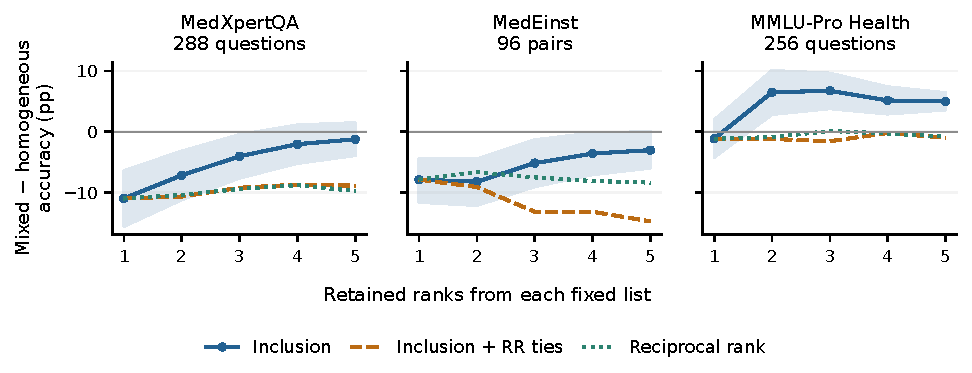
\includegraphics[width=\linewidth]{figures/REPRESENTATION_DEPTH.pdf}
\caption{Fixed-ballot depth replay, two banks per source. All curves coincide at depth one. At depth five, inclusion counts every answer equally; RR and the RR tie-breaker retain rank weights. Left/middle use the original four-model mixture; right uses $M_{44}$ versus $H_G$, as in the separate 720-case design. Bands are secondary paired 95\% intervals for inclusion; other curves are point estimates. $C$ compares paired endpoints, not marginal intervals. MedEinst uses refinements; both other sources use native keys.}
\label{fig:depth_supp}
\end{figure}


\begin{figure}[t]
\centering
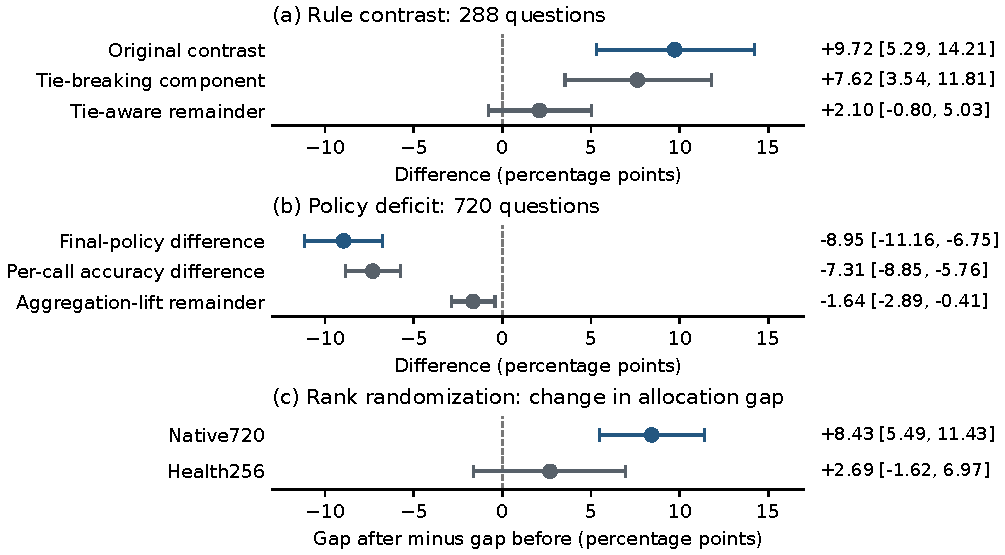
\includegraphics[width=\linewidth]{figures/PRIMARY_EXPLANATIONS.pdf}
\caption{Explanations and a rank intervention. (a,b) Rule and policy decompositions, with paired pointwise 95\% question-bootstrap intervals. Components add within each panel; their correlated intervals must not be added. (c) Paired change in the mixed-minus-Gemma first-choice gap after randomizing ranks, with intervals adjusted across eight endpoints. Both policies worsen; Health's change is unresolved. These exploratory analyses do not isolate a quality-independent lineage effect.}
\label{fig:explanations}
\end{figure}


The separate \path{eleven_review_replay.zip} contains stripped Native288/Native720/Health256 ballots, scored MedEinst rank pools, executable analyses, the exploratory specification, expected outputs and checksums. It contains no question text, credentials or new clinical labels. With Python and NumPy, run \texttt{python3 replay.py --data data --out outputs} and compare the three result files with \path{expected/}. The original eight-check archive remains unchanged. This replay does not regenerate hosted outputs or adjudicate the terminology map.

\subsection{Approval cutoff and tie handling on fixed responses}\label{app:cutoff}

This exploratory challenge asks whether the allocation comparison changes when approval counts only the first two answers rather than all five. It reuses the original Native288, Native720 and Health256 calls, keys, failures, allocations and two-bank averaging. No questions, model calls or clinical labels are added. Approval cutoff is the number of stored positions that receive a vote; it is not the number of answers requested during generation.

For cutoff $k\in\{2,5\}$, give each candidate in the first $k$ positions one vote per call. The uniform version averages all tied maximum-count candidates. The rank-tie version first maximizes approval count, then sums reciprocal ranks from \emph{all five positions} to resolve equal counts. Remaining ties are uniform. Only candidates receiving an approval vote are eligible. Thus the tie-breaker introduces additional preference information; it does not merely choose a deterministic candidate label. Empty allocations score zero. This is not a reproduction of the token-log-probability or additional-model tie procedure of \citet{wang2025ranked}.

Table~\ref{tab:cutoff_absolute} reports all absolute accuracies and tie rates. A tie rate is the proportion of question--bank decisions with multiple winners before the final uniform draw. In particular, Health's two-answer approval gain is not evidence that this policy beats the 68.82\% selected Gemma first-choice reference: its mixed accuracy is only 58.04\%. Adding rank information to break ties raises both allocations, and the mixed-minus-H difference becomes unresolved at $-1.17\ [-4.79,2.44]$ points (nominal paired 95\% interval).

\begin{table}[ht]
\centering\small
\caption{Fixed-response cutoff challenge. All values percent, except mixed-minus-H differences in points. Rank ties use the complete five-position RR score. First-choice and five-answer values reconcile exactly with the retained analyses. These are reused cases, not fresh confirmation.}
\label{tab:cutoff_absolute}
\begin{tabular}{llrrrrr}
\toprule
Source & Rule & H accuracy & M accuracy & M$-$H & H ties & M ties\\
\midrule
Native288 & First &29.86&18.91&$-10.95$&5.90&13.89\\
& Approval 2 &25.55&18.39&$-7.16$&40.45&16.84\\
& Approval 2, rank ties &28.82&18.92&$-9.90$&2.08&0.00\\
& Approval 5 &18.68&17.45&$-1.23$&94.27&66.84\\
& Approval 5, rank ties &29.51&20.66&$-8.85$&2.08&0.35\\
& RR &29.69&19.97&$-9.72$&2.08&0.52\\
\midrule
Native720 & First &35.21&26.26&$-8.95$&4.31&25.49\\
& Approval 2 &31.37&24.70&$-6.67$&37.71&29.24\\
& Approval 2, rank ties &34.93&24.76&$-10.17$&0.83&3.82\\
& Approval 5 &19.49&19.71&$0.22$&95.14&89.17\\
& Approval 5, rank ties &34.34&25.83&$-8.51$&1.04&3.82\\
& RR &34.65&24.86&$-9.79$&1.18&4.65\\
\midrule
Health256 & First &68.82&67.68&$-1.14$&2.54&20.70\\
& Approval 2 &51.56&58.04&$6.48$&60.94&39.06\\
& Approval 2, rank ties &69.43&68.26&$-1.17$&0.98&5.86\\
& Approval 5 &23.48&28.48&$5.00$&99.02&95.70\\
& Approval 5, rank ties &69.04&68.07&$-0.98$&0.98&5.27\\
& RR &69.04&68.26&$-0.78$&0.98&6.05\\
\bottomrule
\end{tabular}
\end{table}

Define $C_2$ as the cutoff-two allocation difference minus the first-choice allocation difference, $U_2$ as the same contrast with rank-resolved approval ties, and $T_2=C_2-U_2$. Resample whole questions 20,000 times within the original source/task strata, seed 20260923; banks remain together. The three $C_2$ contrasts form a three-endpoint family. The six $U_k$ contrasts (two cutoffs, three cohorts) and six $T_k$ contrasts each receive separate Bonferroni interval adjustment. Table~\ref{tab:cutoff_contrasts} shows the cutoff-two results. Native contrasts attenuate and become unresolved; Health retains a positive $C_2$, but not a resolved remainder after tie handling. An unresolved interval does not establish equivalence. Original primary estimates and their prespecified intervals are unchanged; these exploratory families do not retroactively adjust those tests.

\begin{table}[ht]
\centering\small
\caption{Cutoff-two rule contrasts and decomposition, points with family-adjusted 95\% paired intervals. $C_2=T_2+U_2$; correlated intervals must not be added.}
\label{tab:cutoff_contrasts}
\begin{tabular}{lrrr}
\toprule
Source & $C_2$ (three contrasts) & $T_2$ (six contrasts) & $U_2$ (six contrasts)\\
\midrule
Native288 & $3.79\ [-.41,7.93]$ & $2.73\ [-.52,6.00]$ & $1.06\ [-2.75,4.71]$\\
Native720 & $2.28\ [-.45,5.05]$ & $3.50\ [1.50,5.48]$ & $-1.22\ [-3.86,1.42]$\\
Health256 & $7.62\ [2.96,12.21]$ & $7.65\ [3.26,11.97]$ & $-.03\ [-3.42,3.37]$\\
\bottomrule
\end{tabular}
\end{table}

The separate \path{practical_cutoff_replay.zip} supplies stripped ballots, expected results, case vectors, checksums and a standalone program. Run \texttt{python3 replay.py --data data --out outputs}. Its 1,296 independent scalar checks include empty ballots, absent keys, reversed lists and partial lists; baseline means reconcile to $10^{-12}$. Compare both JSON outputs byte-for-byte with \path{expected/}. No network, GPU or model generation is needed.

\subsection{Published aggregation components and tie-choice robustness}\label{app:public_ties}

Could arbitrary uniform ties explain the native mixed-policy deficit? We test this rival without changing any generated answer. The BCV and MRRV classes released with \citet{wang2025ranked}, at commit \texttt{f5bb1c1}, accumulate Borda and reciprocal-rank scores, respectively, then return the first maximum encountered by \texttt{Counter.most\_common(1)}. We execute those classes on all three retained cohorts. Failed empty lists are represented by the source's invalid sentinel and excluded from vote accumulation; their questions remain, and an all-failure allocation scores zero. Native288 keeps its original four-model mixture; Native720 and Health keep their Gemma--Llama mixture.

This is an aggregation-component replay, not a reproduction of the published experiment. Our prompts, models, parser, ten-option questions and stored five-answer lists remain unchanged. The inspected code path has encounter-order tie handling, distinct from the paper-described confidence or extra-model resolution; we do not infer which path produced the authors' original results. Literal MRRV replay preserves floating-point additions. Reversing the eight input lists tests sensitivity to both encounter order and numerical summation, not a new generation order.

\begin{table}[t]
\centering\small
\caption{Published-component replay on existing answers. H/M accuracies are percentages; differences are percentage points. Scheduled-order differences have paired intervals adjusted across six source--rule contrasts. Reversed-order differences are descriptive sensitivity results, not selected policies.}
\label{tab:public_components}
\begin{tabular}{llrrrr}
\toprule
Source & Rule & H & M & M--H [adjusted 95\%] & Reversed\\
\midrule
Native288 & Borda &28.99&21.35&$-7.64\ [-13.83,-1.39]$&$-8.51$\\
& RR &29.69&19.97&$-9.72\ [-15.97,-3.47]$&$-9.72$\\
Native720 & Borda &35.07&25.97&$-9.10\ [-12.78,-5.69]$&$-11.11$\\
& RR &34.72&25.21&$-9.51\ [-13.17,-6.04]$&$-10.28$\\
Health & Borda &69.34&68.95&$-.39\ [-4.49,3.71]$&$-1.17$\\
& RR &68.95&68.55&$-.39\ [-4.69,3.91]$&$-.78$\\
\bottomrule
\end{tabular}
\end{table}

Both native cohorts retain a mixed deficit under both components; Health does not resolve one. Inference resamples questions 20,000 times within source/task, keeping two banks and all policies together, seed20260926. This exploratory six-contrast family does not alter the prespecified primary intervals. Reversing call order changes some estimates but not these observed directions (Table~\ref{tab:public_components}).

We also bound accuracy without specifying a tie-breaking algorithm. For each question--bank allocation, compute the exact set of maximum-score candidates, using rational reciprocal-rank scores. Its lower correctness is one only if gold is the sole maximizer; its upper correctness is one if gold is among the maximizers. Empty allocations have both endpoints zero. Average these endpoints over banks and questions. Subtract H's upper accuracy from M's lower for a lower bound on M--H; subtract H's lower from M's upper for an upper bound. This permits even gold-informed, allocation-specific tie choices: a deliberately generous outer envelope, not an attainable selector. It is not a confidence interval. A negative upper endpoint rules out reversal on these fixed outputs; an envelope containing zero does not demonstrate an operational reversal.

\begin{table}[t]
\centering\small
\caption{Fixed-output mixed-minus-H envelopes over arbitrary score-maximizing tie choices, in percentage points. These are gold-informed bounds, not sampling intervals. Inclusion bounds are deliberately broad because they permit adversarial resolution separately for each allocation.}
\label{tab:tie_envelopes}
\begin{tabular}{lrrrr}
\toprule
Source & First choice & Inclusion & RR & Borda\\
\midrule
Native288 &$[-14.93,-6.08]$&$[-55.38,34.90]$&$[-10.24,-9.20]$&$[-9.90,-6.42]$\\
Native720 &$[-16.04,-1.81]$&$[-61.67,54.24]$&$[-11.46,-8.12]$&$[-12.15,-7.92]$\\
Health &$[-9.38,7.03]$&$[-87.50,86.33]$&$[-3.12,1.56]$&$[-3.91,1.95]$\\
\bottomrule
\end{tabular}
\end{table}

Native720's first-choice upper bound is $-1.81$ points, but its nominal question-bootstrap interval is $[-3.89,.28]$: fixed-sample non-reversal does not establish population-level robustness for every tie policy. The RR/Borda upper-endpoint intervals are $[-10.83,-5.49]$ and $[-10.76,-5.21]$, respectively. Health envelopes cross zero. The results strengthen the native rank-rule deficit against a tie-choice explanation; they do not show that the positive inclusion interaction persists under realistic confidence-based aggregation or fresh prompts.

The \path{tie_policy_replay.zip} archive contains stripped inputs, the pinned source, independent checks and expected per-question outputs. Run \texttt{python3 replay.py --data data --source RankBasedSC.py --out outputs}. All 750 constructed checks and 20,224 actual-output comparisons against an independent literal implementation pass; original uniform-rule means reconcile to $10^{-12}$. No new model calls, labels, cases or costs are introduced. The analysis is post hoc and conditional on retained banks and keys.

